\documentclass[12pt,reqno]{article}

\usepackage[usenames]{color}
\usepackage{amssymb}
\usepackage{graphicx}
\usepackage{amscd}

%\usepackage[colorlinks=true,
%linkcolor=webgreen,
%filecolor=webbrown,
%citecolor=webgreen]{hyperref}
%\definecolor{webgreen}{rgb}{0,.5,0}
%\definecolor{webbrown}{rgb}{.6,0,0}

\usepackage{color}
\usepackage{fullpage}
\usepackage{float}

%\usepackage{psfig}
\usepackage{graphics,amsmath,amssymb}
\usepackage{amsthm}
\usepackage{amsfonts}
\usepackage{latexsym,pifont,fontawesome}
\usepackage{epsf}

\usepackage[a4paper, total={7in, 10.25in}]{geometry}
\setlength{\parindent}{0cm}
\setlength{\parskip}{0.1cm} 

\newcommand{\mathsmaller}[1]{#1}

\newcommand{\citep}{\cite}
\newcommand{\cf}[0]{cf.\ } 
\renewcommand{\emph}[1]{\textit{#1}} 

\theoremstyle{plain}
\newtheorem{theorem}{Theorem}[section]
\newtheorem{lemma}[theorem]{Lemma}
\newtheorem{cor}[theorem]{Corollary}
\newtheorem{prop}[theorem]{Proposition}
\newtheorem{claim}[theorem]{Claim}

\theoremstyle{definition}
\newtheorem{definition}[theorem]{Definition}
\newtheorem{example}[theorem]{Example}
\newtheorem{exercise}[theorem]{Exercise}
\newtheorem{problem}[theorem]{Problem Statement}
%\theoremstyle{remark}
\newtheorem{remark}[theorem]{Remark}

\newcommand{\gkpSI}[2]{\ensuremath{\genfrac{\lbrack}{\rbrack}{0pt}{}{#1}{#2}}} 
\newcommand{\gkpSII}[2]{\ensuremath{\genfrac{\lbrace}{\rbrace}{0pt}{}{#1}{#2}}}
\newcommand{\Iverson}[1]{\ensuremath{\left[#1\right]_{\delta}}} 
\newcommand{\PP}[1]{\ensuremath{\mathbb{P}\left(#1\right)}} 

\usepackage{enumitem}
\setlist[itemize]{leftmargin=0.65in}

\usepackage{upgreek,graphicx}
\renewcommand{\chi}{\scalebox{1.25}{$\upchi$}} 
%\renewcommand{\chi}{\scalebox{1.25}{$\textchi$}} 

%\include{fancysection.sty} 
\usepackage{tikz, blindtext}
\usepackage[utf8]{inputenc}
\usepackage{titlesec}

\newenvironment{vplace}[1][1]
  {\par\vspace*{\stretch{#1}}}
  {\vspace*{\stretch{1}}\par}

%\usepackage[misc]{ifsym} 
\usepackage{epsdice}

\errorcontextlines 10000

\usepackage{intcalc,skak}

\newcommand{\CounterModN}[2]{\value{\intcalcMod{\the#1}{#2}}}
\newcommand{\CounterDiff}[2]{\value{\intcalcSub{\the#1}{#2}}}

\newcommand{\fillchar}[1]{
     \leavevmode\xleaders\hbox{#1}\hfill\kern0pt
}

%\usepackage{tikz} 
%\renewcommand{\textcircled}[2][6pt]{\raisebox{-#1}{\tikz{\node (F) at (0,0) {#2};\draw[thick](F)\circle(#1);}}}

%\titleformat{\section}[block]
%{\normalfont\sffamily\Huge\bfseries}
%{}{0.5em}{\fillchar{\LARGE\ }\hspace{0.5em}\uppercase}
%[\tiny\filleft\rule{\textwidth}{0.1cm}]
%\titlelabel{\hspace{0.1cm}\thetitle}
%\titlespacing{\section}{0pt}{*0}{*0} 

\allowdisplaybreaks

\title{Probability Comprehensive Exam Notes}
\author{Maxie D. Schmidt} 
\date{Revised: \today}

\begin{document}

\vskip -0.45in
\noindent 
\rule{\textwidth}{0.1cm} 

\begin{center} 
{\normalfont\sffamily\Large\bf Probability Comprehensive Exam Notes} \\[0.25cm]  
{\normalfont\sffamily\large Revised: \today}
\end{center}

\noindent 
\rule{\textwidth}{0.1cm} 

\vskip -0.75in
\def\contentsname{\large{Topics Index}}
\setcounter{secnumdepth}{2}
\renewcommand{\baselinestretch}{0.55}\normalsize
\tableofcontents
\renewcommand{\baselinestretch}{1.0}\normalsize

\newpage
\section{Sigma algebras and sets} 

\subsection{Set theory} 

\begin{definition} 
We define the \emph{limit infimum} and \emph{limit supremum} of a sequence of sets by 
\begin{align*} 
\liminf_{n \rightarrow \infty} A_n & = \bigcup_{n \geq 1} \bigcap_{m \geq n} 
     A_m \\ 
     & = \{x: \text{$x$ is in all but finitely many of the $A_n$'s}\} \\ 
\limsup_{n \rightarrow \infty} A_n & = \bigcap_{n \geq 1} \bigcup_{m \geq n} 
     A_m \\ 
     & = \{x: \text{$x$ is in infinitely many of the $A_n$'s}\}. 
\end{align*} 
Observe that for any $N \geq 1$:
$$\limsup_{n \rightarrow \infty} A_n \subseteq \bigcup_{i=N}^{\infty} A_i.$$
The following properties are also apparent:
\begin{itemize} 

\item $\liminf_{n \rightarrow \infty} A_n = 
       \left(\limsup_{n \rightarrow \infty} A_n^c\right)^c$; 
\item $\liminf(A_n) \subseteq \limsup(A_n)$. 

\end{itemize} 
\end{definition} 

\begin{theorem}[Monotonicity of Sequences of Sets and Continuity]
We say that \emph{$A_n$ increases to $A$}, written $A_n \nearrow A$, if 
$A_n \subset A_{n+1}$ for all $n \geq 1$ and $A = \cup_{n \geq 1} A_n$. 
We say that \emph{$A_n$ decreases to $A$}, written $A_n \searrow A$, 
if $A_n \supset A_{n+1}$ for all $n \geq 1$ and $A = \cap_{n \geq 1} A_n$. 
If $A_n \searrow A$, then by continuity we get that 
\[
\lim_{n \rightarrow \infty} A_n = \bigcap_{n \geq 1} A_n. 
\]
\end{theorem} 

For example, if for some sequence of sets $\{E_k\}_{k \geq 1}$, we define 
$F_n := \cup_{m \geq n} E_m$, then we have that $F_n \searrow \cap_{n \geq 1} F_n$. 

\begin{theorem}[Continuity of the Lebesgue measure on monotone sets from Real Analysis]
Let $\{E_k\}$ be a sequence of measurable sets in $\mathbb{R}^n$. 
\begin{itemize} 
\item[(1)] If $E_k \nearrow E$, then $\lim_{k \rightarrow \infty} |E_k| = |E|$; 
\item[(2)] If $E_k \searrow E$ and $|E_k| < \infty$ for some $k$, then 
     $\lim_{k \rightarrow \infty} |E_k| = |E|$. 
\end{itemize} 
\end{theorem} 
\begin{proof}[Proof of 1]
If for some $j \geq 1$, $|E_j| = \infty$ then $|E_k| = \infty$ for all $k \geq j$, and hence 
$|E| = \infty$. Now we can assume that $|E_k| < \infty$ for all $k \geq 1$. 
We write 
\[
E = E_1 \cup (E_2 \setminus E_1) \cup \cdots = E_1 \cup \bigcup_{k \geq 1} (E_{k+1} \setminus E_k). 
\]
Then 
\[
|E| = |E_1| + \sum_{k \geq 1} |E_{k+1} \setminus E_k| = |E_1| + \lim_{n \rightarrow \infty} 
     \sum_{k=1}^n (|E_{k+1}| - |E_k|) = \lim_{n \rightarrow \infty} |E_{n+1}|. 
     \qedhere
\]
\end{proof} 
\begin{proof}[Proof of 2]
We can assume that $|E_1| < \infty$ since otherwise we can truncate the sequence and relabel to 
obtain the same limit. Moreover, we can write $E_1$ as a disjoint union of 
measurable sets: 
\[
E_1 = E \cup \bigcup_{k \geq 1} (E_k \setminus E_{k+1}). 
\]
Now we have that 
\begin{align*} 
|E_1| & = |E| + \sum_{k \geq 1} |E_k \setminus E_{k+1}| \\ 
     & = |E| + \lim_{n \rightarrow \infty} \sum_{k=1}^n (|E_k|-|E_{k+1}|) \\ 
     & = |E| + \lim_{n \rightarrow \infty} (|E_1| - |E_{n+1}|), 
\end{align*} 
which implies the result. 
\end{proof} 

\begin{prop} 
\label{prop_limsups_of_sets_containment_idents} 
For $X_n,Y_n$ random variables and any $a \in \mathbb{R}$, 
$\varepsilon > 0$, we have that 
\begin{align*} 
\limsup \{Y_n > a+\varepsilon\} & \subset \left\{\limsup Y_n > a\right\} 
     \subset \left\{\limsup Y_n > a - \varepsilon\right\} \\ 
\limsup \{Y_n < a-\varepsilon\} & \subset \{\limsup Y_n < a\} \subset 
     \{\limsup Y_n < a+\varepsilon\}, 
\end{align*} 
and that 
\begin{align*} 
\limsup_{n \rightarrow \infty} \{X_n > a+\varepsilon\} & \subseteq 
     \left\{\limsup_{n \rightarrow \infty} X_n > a\right\} \subseteq 
     \limsup_{n \rightarrow \infty} \{X_n > a-\varepsilon\} \\ 
\limsup_{n \rightarrow \infty} \{X_n < a-\varepsilon\} & \subseteq 
     \left\{\limsup_{n \rightarrow \infty} X_n < a\right\} \subseteq 
     \limsup_{n \rightarrow \infty} \{X_n < a+\varepsilon\}. 
\end{align*} 
\end{prop} 

\subsection{Sigma algebras and sigma fields} 

We adopt the conventions that 
\begin{align*} 
\Omega & \equiv \mathrm{sample\ space} = 
  \mathrm{set\ of\ all\ possible\ outcomes}, \\ 
\mathcal{F} & \equiv \mathrm{the\ collection\ of\ all\ events\ (subsets\ 
  of\ the\ sample\ space)} \subseteq \rho(\Omega), 
\end{align*} 
where $\rho(\Omega)$ denotes the \emph{power set of $\Omega$}, or the 
set of all subsets of $\Omega$. 

\begin{definition}[Algebras and Sigma Fields]
The set (of sets) $\mathcal{F}$ is a \emph{algebra} (or \emph{field}) if 
\begin{itemize} 

\item[(1)] $\Omega \in \mathcal{F}$; 
\item[(2)] $A,B \in \mathcal{F} \implies A \cup B \in \mathcal{F}$; 
\item[(3)] $A \in \mathcal{F} \implies A^{c} \in \mathcal{F}$. 

\end{itemize} 
Similarly, the set 
$\mathcal{F}$ is a \emph{$\sigma$-algebra} (or \emph{$\sigma$-field}) if 
\begin{itemize} 

\item[(1)] $\Omega \in \mathcal{F}$; 
\item[(2)] $A_n \in \mathcal{F} 
            \implies \cup_{n \geq 1} A_n \in \mathcal{F}$; 
\item[(3)] $A \in \mathcal{F} \implies A^{c} \in \mathcal{F}$. 

\end{itemize} 
\end{definition} 

Examples of $\sigma$-algebras include the following: 
$\mathcal{F}_1 = \{\varnothing, \Omega\}$ and 
$\mathcal{F}_2 = \rho(\Omega)$, the power set of $\Omega$. 
We have the following consequences of these definitions:
\begin{itemize} 

\item $A,B \in \mathcal{F} \implies A \cap B \in \mathcal{F}$ since 
      $(A \cap B)^c = A^c \cup B^c$; 
\item $A,B \in \mathcal{F} \implies A \setminus B \in \mathcal{F}$; 
\item fields $\subseteq$ $\sigma$-fields; 
\item For $\mathcal{F}$ a $\sigma$-field, $A_n \in \mathcal{F} \implies$ 
      $\cap_{n \geq 1} A_n \in \mathcal{F}$. 

\end{itemize} 

\begin{definition}[$\lambda$-Systems and $\pi$-Systems]
A set $G \subset \rho(\Omega)$ is called a \emph{$\lambda$-system} if 
\begin{itemize} 

\item[(1)] $\Omega \in G$; 
\item[(2)] $A_n \in G$ (disjoint) $\implies$ 
     $\dot{\bigcup}_{n \geq 1} A_n \in G$; 
\item[(3)] $A,B \in G$, $A \subset B$ $\implies$ $B \setminus A \in G$. 

\end{itemize} 
If $C$ is a $\lambda$-system and in addition, 
$C$ is closed under intersections 
(i.e., $A,B \in C$ $\implies$ $A \cap B \in C$), then $C$ is called a 
\emph{$\pi$-system}. 
\end{definition} 

\begin{definition}[Notation]
Let $C$ be a collection of subsets in $\Omega$. Then $\sigma(C)$ is defined 
to be the \emph{smallest $\sigma$-algebra} containing $C$: 
\[
\sigma(C) = \bigcap_{\substack{C \subset \mathcal{F} \\ 
     \mathcal{F} \text{ a\ $\sigma$-algebra}}} \mathcal{F}. 
\]
Similarly, we define $\lambda(C)$ to be the smallest $\lambda$-system 
containing $C$. 
\end{definition} 

\begin{theorem}[Dyukin]
If $C$ is a $\pi$-system, then $\lambda(C) = \sigma(C)$. 
\end{theorem} 

\begin{example}[The Borel Field of $\mathbb{R}$] 
Consider the following sets:
\begin{align*} 
C_1 & = \{(a,b): a < b\} \\ 
C_2 & = \{(a,b]: a < b\} \\ 
C_3 & = \{[a,b]: a < b\} \\ 
C_4 & = \{(-\infty, a]: a \in \mathbb{R}\} \\ 
C_5 & = \{[a,\infty]: a \in \mathbb{R}\} \\ 
C_6 & = \{[a,b]: a,b \in \mathbb{Q}\}. 
\end{align*} 
Then the \emph{Borel field} 
$\beta(\mathbb{R}) = \sigma(C_1) = \cdots = \sigma(C_6)$. It happens that 
all of the $C_i$'s in this example are also examples of $\pi$-systems. 
\end{example} 

\begin{example}[Spring 2019, \#6]
Assume $(\Omega, \mathcal{F}, \mathbb{P})$ is a probability space such that 
there exist $X_1,X_2: \Omega \rightarrow \mathbb{R}$ two independent 
Bernoulli random variables such that $\PP{X_i = 0} = \PP{X_i = 1} = 1/2$. 
Show that $\Omega$ must have at least $4$ elements. 
Give an example with $\Omega$ having $4$ elements together with a 
sigma alpgebra such that on it we can define two independent Bernoulli as 
above. 
Can you generalize this? 
\end{example} 

\newpage 
\section{Probabilities}

\subsection{Definitions and basic properties} 

Throughout we will use the notation that $\Omega$ denotes the 
\emph{sample space} and that $\mathcal{F}$ denotes the $\sigma$-field of 
events. Given a fixed probability $\mathbb{P}$, we will make reference 
to the \emph{probability space} $(\omega, \mathcal{F}, \mathbb{P})$. 

\begin{definition} 
The function $\mathbb{P}: \mathcal{F} \rightarrow [0,1]$ is a 
\emph{probability} if 
\begin{itemize} 

\item $\mathbb{P}(\Omega) = 1$; and 
\item $(A_n)_{n \geq 1} \subset \mathcal{F}$ (disjoint) $\implies$ 
     $\mathbb{P}\left[\cup_{n \geq 1} A_n\right] = \sum_{n \geq 1} 
     \mathbb{P}(A_n)$. 

\end{itemize} 
\end{definition} 
The next properties are apparent from the definition of $P$ as a 
probability function:
\begin{itemize} 

\item $\mathbb{P}(\varnothing) = 0$; 
\item $\mathbb{P}(A^c) = 1 - \mathbb{P}(A)$, $\forall A \in \mathcal{F}$; 
\item $A \subset B$ $\implies$ $\mathbb{P}(B \setminus A) = 
     \mathbb{P}(B) - \mathbb{P}(A)$, since 
     $\mathbb{P}(B) = \mathbb{P}(A) + \mathbb{P}(B \setminus A)$. 

\end{itemize} 

\begin{theorem}[Uniqueness on $\mathbb{R}$]
If $\mathbb{P},\mathbb{Q}$ are two probability measures on $\mathbb{R}$, 
and if $\mathbb{P}(-\infty,x] = \mathbb{Q}(-\infty,x]$ for all 
$x \in \mathbb{R}$, then $\mathbb{P}(A) = \mathbb{Q}(A)$ for all 
$A \in \beta(\mathbb{R})$. 
\end{theorem} 

\begin{definition}[Continuity and Additivity]
A probability $\mathbb{P}$ is \emph{continuous} if 
$A_n \searrow \varnothing$ $\implies$ $\mathbb{P}(A_n) \rightarrow 0$ as 
$n \rightarrow \infty$. The function $\mathbb{P}$ possessing 
\emph{finite additivity} is equivalent to the property that whenever 
$(A_n)_{n \geq 1}$ are disjoint:
\[
\mathbb{P}\left(\bigcup_{i=1}^n A_i\right) = \sum_{i=1}^n \mathbb{P}(A_i). 
\]
On the other hand, \emph{$\sigma$-additivity} is equivalent to 
\[
\mathbb{P}\left(\bigcup_{i=1}^{\infty} A_i\right) = 
     \sum_{i=1}^{\infty} \mathbb{P}(A_i). 
\]
\end{definition} 

\begin{prop}
If $\mathbb{P}$ is finite additive and continuous, then it is 
$\sigma$-additive. 
\end{prop} 

\begin{example}[Properties of Probabilities]
We have the following additional special properties of probability 
function $\mathbb{P}$:
\begin{itemize} 

\item \textbf{Subadditivity:} For any $(A_n) \subseteq \mathcal{F}$, 
     $\mathbb{P}\left(\bigcup_{n \geq 1} A_n\right) \leq 
     \sum_{n \geq 1} \mathbb{P}(A_n)$; 
\item \textbf{Fatou:} If $(A_n) \subseteq \mathcal{F}$ is arbitrary, then 
\[
\mathbb{P}(\liminf A_n) \leq \liminf \mathbb{P}(A_n) \leq 
     \limsup \mathbb{P}(A_n) \leq \mathbb{P}(\limsup A_n). 
\]
\item \textbf{Probabilities on countable sets:} If 
     $\Omega = \{\omega_1, \omega_2, \ldots\}$ is countable, then for any 
     $A \subseteq \Omega$: $\mathbb{P}(A) = \sum_{w_i \in A} 
     \mathbb{P}(\omega_i)$. 

\end{itemize} 
\end{example} 

\subsection{Distribution functions (on $\mathbb{R}$ and $\mathbb{R}^n$)} 

\begin{definition}[Distribution Functions]
If $\mu$ is a probability on $\beta(\mathbb{R})$, then the 
\emph{distribution function of $\mu$} is 
$F_{\mu}(x) := \mu((-\infty,x])$. We have the following properties of the 
distribution function:
\begin{itemize} 

\item[(1)] $\lim\limits_{x \rightarrow -\infty} F_{\mu}(x) = 0$; 
\item[(2)] $\lim\limits_{x \rightarrow \infty} F_{\mu}(x) = 1$; 
\item[(3)] $F_{\mu}$ is non-decreasing; 
\item[(4)] $F_{\mu}$ is right continuous. 

\end{itemize} 
\end{definition}

\begin{theorem}
If $u,v$ are probability measures on $\mathbb{R}$ such that 
$F_u(x) = F_v(x)$ for all $x \in \mathbb{R}$, then 
$u(A) = v(A)$ for all $A \in \beta(\mathbb{R})$. 
\end{theorem} 

\begin{theorem} 
Let $(\Omega, \mathcal{F})$ be a probability space with 
$\mathcal{F} = \sigma(\mathcal{C})$ for $\mathcal{C}$ a $\pi$-system. 
If $P,Q$ are two probabilities on $\mathcal{F}$ such that 
$P(C) = Q(C)$ for all $C \in \mathcal{C}$, then 
$P(A) = Q(A)$ for all $A \in \mathbb{F}$. 
\end{theorem} 

\begin{example}[The Dirac Distribution at a Point]
For a fixed $a \in \mathbb{R}$, we define 
\[
\mu(A) := \delta_a(A) = \begin{cases} 
     1, & a \in A; \\ 0, a \notin A.
     \end{cases}
\]
As we can check $\delta_a$ is a probability measure on $\mathbb{R}$ since 
$\delta_a(\mathbb{R}) = 1$ and $(A_n)$ disjoint $\implies$ 
$\delta_a\left(\cup_{n \geq 1} A_n\right) = \sum_{n \geq 1} \delta_a(A_n)$. 
The distribution function of $\delta_a$, $F_{\delta_a}$, has the following 
plot shape for arbitrary $a \in \mathbb{R}$: 
\begin{center}
\fbox{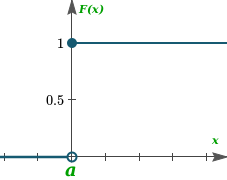
\includegraphics{images/DiracDistFuncFmux.png}}
\end{center} 
\end{example} 

\begin{example}[The Lebesgue Measure on the Unit Interval]
For an interval $[a,b] \subset [0,1]$, we define the 
\emph{Lebesgue measure} by the function 
$\lambda([a,b]) = b-a$ for $0 \leq a < b \leq 1$ where 
$\lambda([0,1]^c) = 0$. Then by integration, we can see that the 
corresponding distribution function satisfies:
\[
F_{\lambda}(x) = \begin{cases} 
     0, & x < 0; \\ 
     x, & 0 \leq x < 1; \\ 
     1, & x \geq 1. 
     \end{cases} 
\]
This distribution function has the following plot: 
\begin{center}
\fbox{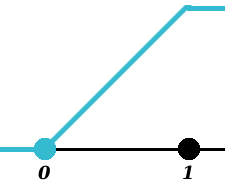
\includegraphics{images/LebesgueDistFuncFlambdax.png}}
\end{center} 
\end{example} 

\begin{example}[Construction of $\mu,F_{\mu}$ from a Function]
Provided that the function $F$ satisfies the four required distrubution 
function properties from the definition above, we can construct a 
probability measure $\mu$ corresponding to this $F$ using the next steps:
\begin{itemize} 

\item Set $\mu((-\infty,x]) := F(x)$. Then 
$\mu((a,b]) = \mu((-\infty,b] \setminus (-\infty,a]) = F(b) - F(a)$ for 
$a < b$. 
\item To handle the closed intervals, take:
\[
\mu([a,b]) = \lim_{n \rightarrow \infty} \mu((a-\frac{1}{n},b]) = 
     \lim_{n \rightarrow \infty} (F(b) - F(a-1/n)) = F(b) - F(a^{-}). 
\]
\item We can apply the \emph{Caratheodory criterion} to see that if 
     $\mu^{\ast}$ is an outer measure, then 
     \[
     \mathcal{A} := \{A \subset \mathbb{R}: \mu^{\ast}(B) = 
     \mu^{\ast}(B \cap A) + \mu^{\ast}(B \setminus A),\ \forall 
     B \in \beta(\mathbb{R})\}, 
     \]
     is a $\sigma$-field. 
\item Finally, we can define 
     $\mu := \mu^{\ast} \Bigr\rvert_{\beta(\mathbb{R})}$. 

\end{itemize}
\end{example} 

\begin{definition}[Probabilities on $\mathbb{R}^n$]
Here, for example, we will select $n := 2$ to illustrate the key properties.
If $\mu$ is a probability on $\mathbb{R}^2$, then its distribution 
function $F_{\mu}(x, y) := \mu((-\infty,x] \times (-\infty,y])$ 
satisfies:
\begin{itemize}

\item[(1)] $\lim_{x,y \rightarrow -\infty} F_{\mu}(x, y) = 0$; 
\item[(2)] $\lim_{\substack{x \rightarrow \infty \\ y \rightarrow \infty}} 
     F_{\mu}(x, y) = 1$; 
\item[(3)] $F_{\mu}$ is non-decreasing in each variable; 
\item[(4)] $F_{\mu}$ is right continuous in each variable. 

\end{itemize} 
\end{definition} 

\begin{example}[Spring 2018, \#7]
Let $F_n,F$ be distribution functions such that $F_n \rightarrow F$ weakly. 
If $F$ is continuois, show that 
\[
\sup_{x \in \mathbb{R}} |F_n(x) - F(x)| \longrightarrow 0. 
\]
\end{example} 

\begin{example}[Fall 2018, \#5]
For distribution functions $F,G$ on the real line, define 
\[
L(F, G) := \inf\left\{\varepsilon>0: \forall t \in \mathbb{R}, 
     F(t) \leq G(t+\varepsilon) + \varepsilon, 
     G(t) \leq F(t+\varepsilon) + \varepsilon\right\}. 
\]
It is known that $L$ is a metric. Prove that $L(F_n, F) \rightarrow 0$ as 
$n \rightarrow \infty$ if and only if $F_n$ converges weakly to $F$. 
\end{example} 

\subsection{Integration review and properties of distribution functions} 

The \emph{mean value theorem} (MVT for derivatives) 
states that if $f$ is defined and continous on $[a,b]$ and 
differentiable on $(a,b)$, then $\exists c \in (a,b)$ such that 
$(b-a) f^{\prime}(c) = f(b) - f(a)$. The 
\emph{intermediate value theorem} (IVT) states that if $f$ is continuous on $[a,b]$, then for 
all $c$ in the range between $f(a)$ and $f(b)$, $\exists x \in (a, b)$ such that $f(x) = c$. 
The \emph{MVT for integrals} states that if $f$ is continuous on $[a,b]$ then $\exists c \in (a,b)$ 
such that $$f(c) = \frac{1}{b-a} \int_a^b f(t) dt.$$ 
Notice that $f$ \textbf{\emph{monotone increasing}} on 
$[a,b]$ $\implies$ $f \in \operatorname{BV}[a,b]$, i.e., $f$ has \emph{bounded variation} on $[a,b]$. 
If $f$ has bounded variation on $[a,b]$, then we can express $f = g-h$ where $g,h$ are both 
bounded and monotone increasing on $[a,b]$. This result is known as the 
\textbf{\emph{Jordan decomposition theorem}}. 
Note that these functions can be extended to 
be monotone increasing on all of $\mathbb{R}$ as well. 
Also, $f$ monotone increasing implies that $f$ is differentiable a.e., $f^{\prime} \geq 0$, and 
$\int_a^b f^{\prime}(t) dt \leq f(b)-f(a)$ for all $a < b$. 

\begin{prop}[Monotone increasing function properties]
If $f$ is \emph{monotone increasing}, then 
\begin{itemize}
\item[(a)] $f$ has at most countably many points of discontinuity. 
\item[(b)] $f$ is differentiable a.e.
\item[(c)] $f^{\prime}$ is a measurable function.
\item[(d)] $f^{\prime} \in L^1$ and we have the FTC as an upper bound: 
     $0 \leq \int_a^b f^{\prime} \leq f(b) - f(a)$.
\end{itemize} 
\end{prop} 
\noindent 
\textbf{Nested characterizations:} 
We say that $f$ is \emph{Lipschitz on $[a,b]$} if there exists a $K > 0$ (where $K$ is 
independent of all $x,y \in [a,b]$) such that 
$|f(x)-f(y)| \leq K \cdot |x-y|$ for all $x,y \in [a,b]$. 
We have the next important nested inclusion of function types. Here, 
$C^1$ denotes the set of functions with one continuous derivative:
\[
C^1[a,b] \subsetneq \operatorname{Lip}[a,b] \subsetneq \operatorname{AC}[a,b] \subsetneq 
     \operatorname{BV}[a,b] \subsetneq L^{\infty}[a,b]. 
\] 
Typical counter examples to these types of functions are $\sqrt{x}$ or are of the form 
$f(x) = x^a \sin(1 / x^b)$. 

\subsection{The product construction} 

\begin{definition}[Products]
Suppose that $(\Omega_1, \mathcal{F}_1, P_1)$ and 
$(\Omega_1, \mathcal{F}_2, P_2)$ are two probability spaces. 
Then the \emph{product construction} between these two spaces 
corresponds to taking $\Omega := \Omega_1 \times \Omega_2$, 
$\mathcal{F} := \mathcal{F}_1 \otimes \mathcal{F}_2 := \sigma( 
 \{A \times B: A \in \mathcal{F}_1, B \in \mathcal{F}_2\})$, and the 
tensor of the probabilities as $\mathbb{P} := P_1 \otimes P_2$, where 
$\mathbb{P}(A \times B) = P_1(A) \cdot P_2(B)$. 
\end{definition} 

\begin{example}[Spring 2019, \#7]
If $X,Y$ are two random variables such that $X \geq Y$ and $X,Y$ have the 
same distribution, then $X = Y$ almost surely. 
\end{example} 

\newpage 
\section{Independence} 

\subsection{Basics and preliminaries}

For our probability space $(\Omega, \mathcal{F}, \mathbb{P})$, in general for 
any $A,B \in \mathcal{F}$, the conditional probability of $A$ given $B$ has 
occurred is 
\[
\mathbb{P}[A|B] = \frac{\mathbb{P}[A \cap B]}{\mathbb{P}[B]}. 
\]
As a notion of \emph{independence} of the random variables $A$ and $B$, we want that 
observing $B$ does not affect the probability of $A$, i.e., that 
$\mathbb{P}[A|B] = \mathbb{P}[A]$ provided that $\mathbb{P}[B] \neq 0$. 
This is equivalent to the condition that $\mathbb{P}[A \cap B] = \mathbb{P}[A] \cdot \mathbb{P}[B]$, 
which holds even when $\mathbb{P}[B] = 0$. 
\emph{Thus we take this property as our definition of independence: } 
\fbox{$\mathbb{P}[A \cap ] = \mathbb{P}[A] \cdot \mathbb{P}[B]$}. 

\begin{example} 
First, if $A := \varnothing,\Omega$, then $A,B$ are always independent for any $B \in \mathcal{F}$. 
We have that if $A,B$ are independent, then $A^C,B$ are independent. We can prove this fact using the 
following logic:
\begin{align*} 
\mathbb{P}(A^C \cap B) & = \mathbb{P}(B \setminus A) = \mathbb{P}(B) - \mathbb{P}(A \cap B),\ 
     \text{ by independence, } \\ 
     & = \mathbb{P}(B) - \mathbb{P}(A) \mathbb{P}(B) = (1-\mathbb{P}(A)) \mathbb{P}(B) \\ 
     & = \mathbb{P}(A^C) \mathbb{P}(B). 
\end{align*} 
So to summarize, any of the elements of $\{\varnothing,\Omega,A,A^C\}$ are independent of any in 
$\{\varnothing,\Omega,B,B^C\}$ whenever $A,B$ are independent. 
\end{example} 
We generalize to the independence of a set of random variables by defining that 
$A_1,A_2,\ldots,A_n$ are independent if $\forall 1 \leq i_1 < i_2 < \cdots < i_k \leq n$ (with 
$2 \leq k \leq n$) $\implies$ 
\[
\mathbb{P}(A_{i_1} \cap \cdots \cap A_{i_k}) = \mathbb{P}(A_{i_1}) \cdots \mathbb{P}(A_{i_k}). 
\]
Note that this definition implies pairwise independence, but is actually a much stronger 
requirement. For example, $A,B,C$ are independent if each of 
$\PP{A \cap B} = \PP{A} \PP{B}$, $\PP{A \cap C} = \PP{A} \PP{B}$, 
$\PP{B \cap C} = \PP{B} \PP{C}$, and $\PP{A \cap B \cap C} = \PP{A} \PP{B} \PP{C}$. 
In general, for $I$ some indexing set, we make the next definition: 
$(\mathcal{F}_i)_{i \in I}$ are independent if $\forall i_1,\ldots,i_n \in I$ (distinct) with 
$A_{i_j} \in \mathcal{F}_{i_j}$ we have 
\[
\PP{A_{i_1} \cap \cdots \cap A_{i_n}} = \prod_{j=1}^n \PP{A_{i_j}}. 
\]

\begin{theorem}[Generation Theorem] 
For any $i \in I$, assume that $\mathcal{F}_i \in \sigma(C_i)$ for $C_i$ always a $\pi$-system. 
Then $(\mathcal{F}_i)_{i \in I}$ are independent if and only if $\forall i_1,\ldots,i_n \in I$ 
(distinct), and with $A_{i_j} \in C_{i_j}$, then 
$\PP{C_{i_1} \cap \cdots \cap C_{i_n}} = \PP{C_{i_1}} \cdots \PP{C_{i_n}}$. 
\end{theorem} 

\begin{cor}[Grouping Theorem] 
If $(\mathbb{F}_i)_{i \in I}$ are independent, and if $\{I_j\}_{j \in J}$ partition $I$ as 
$I = \dot{\cup}_{j \in J} I_j$, and if $\sigma_j := \sigma(\{\mathcal{F}_i: i \in I_j\})$, 
then the $(\sigma_j)_{j \in J}$ are independent. 
\end{cor} 

\begin{example}[Independent Groupings] 
Suppose that the sequence of $(A_n)_{n \geq 1}$ are independent. Then for 
\begin{align*} 
B_1 & := A_1 \cup A_3 \cup A_5 \cup A_7 \cup \cdots \\ 
B_2 & := (A_2 \cap A_4 \cap A_6) \cup (A_8 \cap A_{10} \cap A_{12}) \cup \cdots \\ 
C_1 & := A_1 \cup A_4 \cup A_7 \cup A_{10} \cup \cdots \\ 
C_2 & := (A_2 \cap A_5) \cup (A_8 \setminus A_{11}) \cup \cdots \\ 
C_3 & := (A_3 \setminus A_6) \cup (A_9 \setminus A_{12}) \cup \cdots , 
\end{align*} 
we have that $B_1,B_2$ and $C_1,C_2,C_3$ are each independent from the ``grouping'' 
corollary above. 
\end{example} 

\begin{example}[A Set Independent of Itself] 
Observe that $A$ is independent of itself (henceforth, a.s. constant per exam 2), then 
$\PP{A} \in \{0,1\}$. This happens because of our independence requirement that 
$\PP{A} = \PP{A \cap A} = \PP{A}^2 \implies \PP{A} \in \{0,1\}$. 
\end{example} 

\begin{example}[A Three-Variable Proof] 
If $A,B,C$ are independent, then we can prove also that $A^C,B,C$ are independent: 
\begin{align*} 
\PP{A^C \cap B \cap C} & = \PP{(B \cap C) \setminus A} = \PP{B \cap C} - \PP{B \cap C \cap A} \\ 
     & = \PP{B} \PP{C} - \PP{B} \PP{A} \PP{C} = (1-\PP{A}) \PP{B} \PP{C} \\ 
     & = \PP{A^C} \PP{B} \PP{C}. 
\end{align*} 
\end{example} 

\begin{example}[Fall 2016, \#6]
Let $\{A_n\}$ be an infinite collection of independent events. 
Suppose that $\PP{A_n} < 1$ for every $n \geq 1$. Show that 
$\PP{A_n, i.o.} = 1$ if and only if $\PP{\cup A_n} = 1$. 
\end{example} 

\subsection{Key examples and results} 

\begin{theorem}[Kolmogorov's $0-1$ Law] 
Let $(\mathcal{F}_n)_{n \geq 1}$ be an infinite sequence of $\sigma$-fields. The corresponding, 
so-called \emph{tail field} is 
\[
T := \bigcap_{n \geq 1} \sigma(\mathcal{F}_n, \mathcal{F}_{n+1}, \ldots), 
\]
where the sets $\sigma(\mathcal{F}_n, \mathcal{F}_{n+1}, \ldots)$ are decreasing with $n$. 
If the $(\mathcal{F}_n)_{n \geq 1}$ are independent, then $\PP{A} \in \{0,1\}$ for all 
$A \in T$. 
As a consequence of this phenomenon, we observe that if $(A_n)_{n \geq 1}$ are independent, then 
\begin{itemize} 

\item[(1)] $\PP{\limsup_{n \rightarrow \infty} A_n} \in \{0,1\}$; and 
\item[(2)] $\PP{\liminf_{n \rightarrow \infty} A_n} \in \{0,1\}$. 

\end{itemize} 
\end{theorem} 

\begin{theorem}[Borel-Cantelli Lemma] 
If $(A_n)_{n \geq 1}$ is such that $\sum_{n \geq 1} \PP{A_n} < \infty$, then 
importantly, $\PP{\limsup_{n \rightarrow \infty} A_n} = 0$. This observation 
is later employed to guarantee almost sure convergence of the $A_n$ to zero 
provided that the latter sum converges. Secondly, if $(A_n)_{n \geq 1}$ are 
independent, then 
\[
\sum_{n \geq 1} \PP{A_n} = +\infty \implies \PP{\limsup_{n \rightarrow \infty} A_n} = 1. 
\]
\end{theorem} 

\noindent 
\textbf{Proof Note:} We can utilize the trick that for any set $A \in \mathbb{F}$, 
$\PP{A^C} = 1 - \PP{A} \leq e^{-\PP{A}}$, which is essentially the same as 
saying that $1-x \leq e^{-x}$ whenever $x \in [0, 1]$. 

\begin{example}[Spring 2019, \#2]
If $(X_n)_{n \geq 1}$ is a sequence of random variables, then there exists a 
sequence $(c_n)_{n \geq 1}$ with $c_n \rightarrow \infty$ such that 
\[
\PP{\lim_{n \rightarrow \infty} \frac{X_n}{c_n} = 0} = 1. 
\]
\end{example} 

\begin{example}[Spring 2018, \#8]
Let $(X_n)_{n \geq 1}$ be an iid sequence of random variables. Show that 
$E[X_1^2] < \infty$ if and only if for every $c > 0$, 
$\PP{|X_n| \geq c\sqrt{n} \text{ infinitely often}} = 0$. 
\end{example} 

\begin{example}[Preview of Independent Bernoulli Random Variables] 
For $n \geq 1$, let $X_n \sim \operatorname{Bernoulli}(p_n)$ so that 
$\mathbb{P}(X_n = 1) = p_n$ and $\mathbb{P}(X_n = 0) = 1-p_n$. Then 
we claim that $X_n \xrightarrow{a.s.} 0$ $\iff$ 
$\sum_{n \geq 1} p_n < \infty$. This is true since if the right-hand-side 
sum converges then 
\[
\sum_{n \geq 1} \mathbb{P}(X_n = 1) = \sum_{n \geq 1} \mathbb{P}( 
     |X_n - 0| > \varepsilon) < \infty, 
\]
so that by Borel-Cantelli 
$\limsup_{n \rightarrow \infty} \mathbb{P}(|X_n| > \varepsilon) = 0$. 
\end{example} 

\begin{example}
If $X_1,\ldots,X_n$ are independent, then for 
$\phi_1,\ldots,\phi_n: \mathbb{R} \rightarrow \mathbb{R}$ measurable, 
the random variables $Y_i := \phi_i(X_i)$ are still independent. 
Why is this the case? 
\[
\{Y_i \in A_i\} = \{\phi_i(X_i) \in A_i\} = \{X_i \in \phi_i^{-1}(A_i)\}, 
\]
where the $\phi_i^{-1}(A_i)$'s are measurable. Hence, the $Y_i$'s are 
independent as well. 
\end{example} 

\newpage 
\section{Random variables} 

\subsection{Definitions and basic properties} 

\begin{definition} 
A function $X: \Omega \rightarrow \mathbb{R}$ defined on the sample space is a 
\emph{random variable} if $X^{-1}(A) \in \mathcal{F}$ for all $A \in \beta(\mathbb{R})$. 
Here, we define $X^{-1}(A) := \{\omega: X(\omega) \in A\} = \{X \in A\}$ where the second 
set notation is used more ``loosely'' as a simplification to use as a nice tool for 
understanding. We immediately get the following properties which are apparent given 
our nice new notation for expressing the meaning of a r.v. $X$:
\begin{itemize} 

\item[(1)] $X^{-1}\left(\bigcup_{i \in I} A_i\right) = \bigcup_{i \in I} X^{-1}(A_i)$; 
\item[(2)] $\left\{X \in \bigcap_{i \in I} A_i\right\} = \bigcap_{i \in I} \{X \in A_i\}$; and 
\item[(3)] $\{X \in A^C\} = \{X \in A\}^C$, or in other words, $X^{-1}(A^C) = X^{-1}(A)^C$. 

\end{itemize} 
For any fixed random variable $X$, we get a corresponding \emph{probability measure} 
$\mu_X$ defined by 
\[
\mu_X(B) = \PP{X \in B} = \PP{X^{-1}(B)},\ \forall B \in \beta(\mathbb{R}). 
\]
\textbf{Generalizations:} 
We can extend this notion more generally by setting $(\Omega,\mathcal{F}) \mapsto (S, \varsigma)$, with 
$\mathcal{F},\varsigma$ both $\sigma$-fields. In particular, a $S$-valued random variable is a 
function $X: \Omega \rightarrow S$ such that $\{X \in A\} \in \mathcal{F}$ for all $A \in \varsigma$. 
The next couple of results fill in some key details for extended random variables of this type. 
\end{definition} 

\begin{prop}
If $X: \Omega \rightarrow S$ is a random variable, and $\varsigma$ a $\sigma$-field, then 
$\mathcal{F}_X = X^{-1}(\varsigma) = \{X^{-1}(A): A \in \varsigma\}$ is a $\sigma$-field. 
Moreover, if $X: \Omega \rightarrow S$, with $\varsigma = \sigma(\mathcal{C}^{\prime})$, then 
$\sigma(X^{-1}(\mathcal{C}^{\prime})) = X^{-1}(\varsigma) = X^{-1}(\sigma(\mathcal{C}^{\prime}))$. 
\end{prop} 

\begin{cor}[Characterization for the $\mathbb{R}$ Case]  
If $S = \sigma(\mathcal{C}^{\prime})$, then $X: \Omega \rightarrow S$ is a random variable 
if and only if $X^{-1}(A) \in \mathcal{F}$ for all $A \in \mathcal{C}^{\prime}$. In the 
real-field case, $X: \Omega \rightarrow \mathbb{R}$ is a random variable if and only if 
$\forall x \in \mathbb{R}$, the sets $\{X \leq x\} \in \mathcal{F}$. 
\end{cor} 

\begin{prop}[Useful General Facts for the Real Case] 
We have the next several observations which are collected together here as a matter of 
reference and completeness:
\begin{itemize} 

\item[(1)] If $X_1,\ldots,X_n$ are random variables on $\Omega$, then the tuple 
     $X \equiv (X_1,\ldots,X_n): \Omega \rightarrow \mathbb{R}^n$ is a 
     $\mathbb{R}^n$-valued random variable; 
\item[(2)] If $g: \mathbb{R}^n \rightarrow \mathbb{R}$ is a measurable function, i.e., if 
     $g^{-1}(A) \in \beta(\mathbb{R}^n)$ for all $A \in \beta(\mathbb{R})$, then 
     $g(X_1,\ldots,X_n)$ is a random variable when the $X_i$'s are; 
\item[(3)] If $g: \mathbb{R}^n \rightarrow \mathbb{R}$ is continuous, then $g$ is measurable; 
\item[(4)] Examples of measurable functions on $\mathbb{R}^2$ include: 
     $g(x, y) = x+y, x-y, xy, \frac{x}{y}$ ($y \neq 0$), and $g(x, y) = \chi_A(x) \chi_B(y)$ for 
     $A,B \in \beta(\mathbb{R})$ are all measurable, let's say where they are defined. 

\end{itemize} 
\end{prop} 

\begin{example}[Limits] 
If $\{X_n\}_{n \geq 1}$ is any sequence of random variables, then 
$$Y := \inf X_n, \sup X_n, \liminf X_n, \limsup X_n,$$ are all 
random variables. 
\end{example} 

\begin{example}[Spring 2017, \# 4]
Let $X,Y$ be independent, and suppose that each has a uniform distribution 
on $(0,1)$. Let $Z := \min(X, Y)$. Find the density $f_Z(z)$ for $Z$. 
\end{example} 

\subsection{Independence} 

\begin{definition}[Independence] 
If $(X_i)_{i \in I}$ are random variables on the probability space 
$(\Omega, \mathcal{F}, \mathbb{P})$, we say that the sequence is independent 
if $(\mathcal{F}_{x_i})_{i \in I}$ are independent. Here, we write 
$\mathcal{F}_{x_i} = \{X_i^{-1}(A): A \in \beta(\mathbb{R})\}$. \\ 
\textbf{The next is a key characterization concerning the independence of 
random variables:} \\ 
$(X_i)_{i \in I}$ are independent if whenever $i_1,\ldots,i_n \in I$ are 
distinct, 
\[
\PP{X_{i_1} \leq x_{i_1},\ldots,X_{i_n} \leq x_{i_n}} = 
     \PP{X_{i_1} \leq x_{i_1}} \cdots \PP{X_{i_n} \leq x_{i_n}}, 
\]
for any $x_{i_1},\ldots,x_{i_n} \in \mathbb{R}$. 
\end{definition} 

\begin{prop}
If $X_1,\ldots,X_n$ are independent random variables and $g_1,\ldots,g_n$ are 
Borel measurable functions, then $g_1(X_1),\ldots,g_n(X_n)$ are also independent. 
\end{prop} 

\begin{prop}
If $X,Y$ are independent random variables with both $E[X],E[Y] < \infty$, then 
$E[|XY|] < \infty$ and $E[XY] = E[X]E[Y]$. 
\end{prop} 

\begin{remark}[Orthogonal Random Variables]
Random variables $X,Y$ such that $E[XY] = E[X]E[Y]$ are called \emph{orthogonal}. 
It is clear from the above that independent random variables with finite expectation 
are orthogonal. We also have that if $X_1,\ldots,X_n$ are random variables with 
finite variance, and if $X_1,\ldots,X_n$ are pairwise orthogonal, then 
\[
\operatorname{Var}(X_1+\cdots+X_n) = \operatorname{Var}(X_1) + \cdots + 
     \operatorname{Var}(X_n). 
\]
\end{remark} 

\begin{example}[Spring 2018, \#3]
Let $X,T$ be random variables with $E[X], E[Y] < \infty$. Prove that if 
$E[X|Y]=Y$ and $E[Y|X] = X$, then $X = Y$ a.s.
\end{example} 

\begin{example}[Fall 2018, \#2]
Suppose $X_1,\ldots,X_n$ are iid random variables such that 
$\PP{X_j = +1} = \PP{X_j = -1} = 1/2$. Let $S_k := X_1+\cdots+X_k$ for 
$1 \leq k \leq n$. Prove that 
\[
\PP{\max_{1 \leq k \leq n} S_k \leq \ell} = 2\PP{S_n > \ell} + 
     \PP{S_n = \ell}. 
\]
\end{example} 

\begin{example}[Spring 2019, \#8]
Assume that $X_1,X_2,\ldots,X_n$ are iid with density $f(x) = \frac{2}{x^3}$ 
for $x \geq 1$ and $0$ otherwise. Define 
\[
M_n := \frac{1}{n} \max\{X_1, \sqrt{2} X_2,\ldots, \sqrt{n} X_n\}.
\]
Show that $X_n$ converges in distribution and find the limit. 
\end{example} 

\subsection{Conditional expectation} 

\begin{example}[Fall 2018, \#8]
Let $X$ and $Y$ be two independent and positive random variables with 
respective density $F_X,f_Y$, and let $g: (0, \infty) \rightarrow (0, \infty)$ 
be a bounded Borel function. Find 
\[
E\left[g\left(\frac{X}{Y}\right) \Bigr\rvert Y\right], 
\]
the conditional expectation of $g(X/Y)$ given $Y$, and then infer that 
$V := X/Y$ has a density that you will identify. 
\end{example} 

\begin{example}[Fall 2018, \#9]
Let $X,Y,Z$ be random variables such that $(X,Z)$ and $(Y,Z)$ are 
identically distributed. Let $f: \mathbb{R} \rightarrow \mathbb{R}$ be 
a Borel function such that $f(X)$ is integrable. 
\begin{itemize} 

\item[(i)] Show that $E[f(X) | Z] = E[f(Y) | Z]$, a.s.; and 
\item[(ii)] Let $T_1,\ldots,T_n$ be iid random variables with finite 
     first moment, and let $T = T_1+\cdots+T_n$. Using (i), show that 
     \[
     E[T_1|T] = \frac{T}{n}. 
     \]
     
\end{itemize} 
\end{example} 

\subsection{Common distributions}

\begin{definition}
We introduce models for some of the most common discrete probability distributions 
below. In each of the following cases, $X: \Omega \rightarrow \mathbb{R}$ (or 
possibly $\mathbb{R}^n$) is a random variable, and it's probability 
distribution, or measure function which is what varies from case to case, 
is denoted by $\mu_X$: 
\begin{itemize} 

\item \textbf{Bernoulli:} For a fixed probability $p \in (0, 1)$, we say that 
     $X \sim \operatorname{Bernoulli}(p)$ if $\PP{X = 1} = p$ and $\PP{X = 0} = 1-p$. 
     Here, we express the measure function by $\mu_X = p\delta_1 + (1-p)\delta_0$, where 
     $$\delta_a(A) = \begin{cases} 1, & a \in A; \\ 0, & a \notin A, \end{cases}$$ is 
     the \emph{Dirac delta function}. Indeed, we can see that this expansion is 
     correct since 1) $\mu_X$ is additive (because the $\delta_i$'s are); and 
     2) it is a probability measure as 
     $\mu_X(\mathbb{R}) = p \delta_1(\mathbb{R}) + (1-p) \delta_0(\mathbb{R}) = 1$. 
     It is standard information that $E[X] = p$, and $\operatorname{Var}(X) = pq$, where 
     $q = 1-p$ is the flipped probability for the distribution. 
     Note that a sum of $n$ iid Bernoulli random variables with parameter 
     $p$ have mean $\mu = np$ and variance $np(1-p)$. 
\item \textbf{Uniform:} $X \sim \operatorname{Uniform}$ (on a finite, or countable set) 
     if $S = \{x_1,\ldots,x_n\}$ and we have that $\mu_X(\{x_1\}) = \cdots = \mu_X(\{x_n\}) = \frac{1}{n}$. 
     Alternately, we can state this condition as $X: \Omega \rightarrow \mathbb{R}$ is uniform on $S$ 
     provided that $\PP{X = x_1} = \cdots = \PP{X = x_n} = \frac{1}{n}$. 
\item \textbf{Geometric:} $X \sim \operatorname{Geom}(p)$, which models 
     $$X := \#\text{ flips in a sequence of coin tosses until the first $H$ occurs}.$$ 
     We have: $\PP{X = k} = p(1-p)^{k-1}$ for any natural numbers $k \geq 1$. 
\item \textbf{Binomial:} $X \sim \operatorname{Binomial}(n, p)$, where $X$ models 
     $X := \#\text{ $H$'s in $n$ coin flips}$, and is such that 
     $\PP{X = k} = \binom{n}{k} p^k(1-p)^{n-k}$ for $0 \leq k \leq n$. 
     We can show that $E[X] =: \mu = np$, and 
     $\operatorname{Var}(X) = np(1-p)$. 
\item \textbf{Poisson:} $X \sim \operatorname{Poisson}(\lambda)$, for $\lambda > 0$, if 
     for all integers $k \geq 0$: $\PP{X = k} = e^{-\lambda} \frac{\lambda^k}{k!}$. The 
     \emph{Poisson distribution} naturally arises as the limit of a 
     binomial distribution when the expected number of successes stays 
     fixed at $\lambda$: namely, the limiting distribution of 
     $X \sim \operatorname{Binomial}(n, \lambda / n)$ as 
     $n \rightarrow \infty$. It can be verified that if $X$ is 
     Poisson with parameter $\lambda > 0$, then 
     $E[X] = \lambda$, $E[X(X-1)] = \lambda^2$, and 
     $\operatorname{Var}(X) = E[X^2]-E[X]^2 = \lambda$. 

\end{itemize} 
\end{definition} 

\begin{example}[Preview of Continuous Random Variable Distributions] 
$X$ is a \emph{continuous random variable} if its probability measure, $\mu_X$, has 
a consistent density function. Namely, $f$ satisfying $f \geq 0$, 
$\int_{\mathbb{R}} f = 1$, and where $\mu_X(A) = \int_A f(x) dx$. The following 
listing provides a brief overview of the properties of several of the most common 
cases we will see: 
\begin{itemize} 

\item \textbf{Exponential:} With the construction of this model distribution, we have that 
     the density function is non-zero, and equal to $f(x) = \lambda e^{-\lambda x}$, iff and only 
     if $x > 0$. It is defined to be zero otherwise. Here, to ensure that we get a resulting 
     probability measure, the requirement is that $\lambda > 0$, for example as in other 
     instances in the next sections, with $\lambda := 1$. 
     Note that since we have that $\PP{X \geq t} = e^{-\lambda t}$, 
     $\forall t \geq 0$, we can compute that 
     \begin{align*} 
     E[X] & = \int_0^{\infty} \lambda x e^{-\lambda x} dx = \frac{1}{\lambda} \\ 
     E[X^2] & = \frac{2}{\lambda^2} \\ 
     \operatorname{Var}(X) & = E[X^2]-E[X]^2 = \frac{1}{\lambda^2}. 
     \end{align*} 
     The exponential distribution has the so-called 
     \emph{loss-of-memory property}, which is to say that for all 
     $s,t \geq 0$, $\PP{X \geq s+t | X \geq s} = \PP{X \geq t}$. 
\item \textbf{Uniform:} A.k.a., the non-discretized version of a uniformly distributed random 
     variable on some $[a,b] \subset \mathbb{R}$. Then the density and cumulative density 
     functions respectively have the formulas: 
     \begin{align*} 
     f(x) & = \begin{cases} 
          \frac{1}{b-a}, & x \in [a,b]; \\ 
          0, & \text{ otherwise, } 
          \end{cases} \\ 
      F(x) & = \begin{cases} 
           0, & x < a; \\ 
           \frac{x-a}{b-a}, & x \in [a,b); \\ 
           1, & x \geq b. 
           \end{cases} 
     \end{align*} 
     Here, we have that $\mu = \frac{1}{2}(a+b)$ and 
     $\sigma^2 = \frac{(b-a)^2}{12}$, where the density function can be 
     rewritten as 
     \[
     f(x) = \begin{cases} 
          \frac{1}{2\sigma\sqrt{3}}, & -\sigma\sqrt{3} \leq x-\mu \leq 
               \sigma\sqrt{3} \\ 
          0, & \text{ otherwise. }
          \end{cases} 
     \]
\item \textbf{Standard Normal:} $f(z) = \frac{1}{\sqrt{2\pi}} e^{-z^2 / 2}$. 
     See Section \ref{Section_NormalRVs} for a substantially complete treatment. 
     Note that $X_i \sim N(0, 1)$ $\implies$ 
     $Y := \sum_{i=1}^n \alpha_i X_i \sim N(0, \alpha_1^2+\cdots+\alpha_n^2)$. 
     If $X_i \sim N(\mu_j, \sigma_j^2)$, then 
     $Y := \sum_{i=1}^n X_i \sim N(\mu_1+\cdots+\mu_n, \sigma_1^2+\cdots\sigma_n^2)$. 
     If $X_i \sim N(0, 1)$, then $Z_n = X_1+\cdots+X_n$ has the same 
     distribution as $\sqrt{n} Z$. 
\item \textbf{Gamma:} For parameters $\lambda,\alpha > 0$, we say that 
     $X \sim \operatorname{Gamma}(\lambda, \alpha)$ if 
     $f(x) = \frac{\lambda^{\alpha}}{\Gamma(\alpha)} x^{\alpha-1} 
      e^{-\lambda x}$ for $x > 0$. Here, the \emph{gamma function} is 
     defined by the usual integral 
     $\Gamma(\alpha) = \int_0^{\infty} x^{\alpha-1} e^{-x} dx$. 
     We have the following properties of compositite (sum) distributions 
     which result in gamma-distributed random variables: 
     \begin{itemize} 
     
     \item[(G.0)] If $\alpha = 1$ then 
          $\operatorname{Gamma}(\lambda, 1) \equiv 
           \operatorname{Exp}(\lambda)$ is the exponential distribution;   
     \item[(G.1)] If $X_1,\ldots,X_n$ are iid with 
          $X_1 \sim \operatorname{Exp}(\lambda)$, then 
          $X_1+\cdots+X_n \sim \operatorname{Gamma}(\lambda, n)$; 
     \item[(G.2)] More generally, if $X_1,\ldots,X_n$ are iid random 
          variables with $X_i \sim \operatorname{Gamma}(\lambda, \alpha_i)$, 
          then 
          $X_1+\cdots+X_n \sim \operatorname{Gamma}(\lambda, \alpha_1+\cdots+\alpha_n)$' 
     \item[(G.3)] If $Z \sim N(0, 1)$ is standard normal, then 
          $Z^2 \sim \operatorname{Gamma}\left(\frac{1}{2}, \frac{1}{2}\right)$; 
     \item[(G.4)] If $n \geq 1$ is an integer then the distribution 
          $\operatorname{Gamma}\left(\frac{1}{2}, \frac{n}{2}\right)$ is called the 
          \emph{$\chi^2$-distribution with $n$ degrees of freedom}, which also 
          corresponds to the distribution of $Z_1^2+\cdots+Z_n^2$ where 
          $Z_1,\ldots,Z_n$ are iid standard normal random variables. 
     
     \end{itemize} 

\end{itemize} 
\end{example} 

\begin{exercise}
Show that if $X \sim \operatorname{Exp}(\lambda = 1)$ and 
$U := e^{-X}$ that $U \sim \operatorname{Uniform}(0, 1)$. 
\end{exercise} 
\begin{proof}[Solution to Exercise]
We know by a fact that the $n^{th}$ moment of the uniform distribution on $[a,b]$ is 
given by the following equation for $Y \sim \operatorname{Uniform}(a, b)$: 
$$E[Y^n] = \frac{1}{n+1} \sum_{k=0}^n a^k b^{n-k}.$$
This implies that the $n^{th}$ moment for $n \geq 1$ of $\operatorname{Uniform}(0, 1)$ is 
given by $\frac{1}{n+1}$. Thus it suffices to show that the random variable $U$ defined above 
has $n^{th}$ moments precisely equal to $\frac{1}{n+1}$ for all $n \geq 1$. 
To find the expectations $E[U^n] = E[e^{-nX}]$, we can use the composition formula which states 
that $E[\phi(X)] = \int \phi(x) \mu_X(dx)$. In particular, we have that 
\begin{align*} 
E[U^n] & = \int_0^{\infty} \lambda e^{-\lambda x} e^{-nx} dx = \int_0^{\infty} \lambda e^{-(\lambda+n) x} dx \\ 
     & = -\frac{\lambda}{n+\lambda} e^{-(n+\lambda)x} \Biggr\rvert_{0}^{\infty} = 
     \frac{\lambda}{n+\lambda} \longmapsto \frac{1}{n+1}, 
\end{align*} 
when $\lambda := 1$. 
\end{proof}

\begin{example}[Spring 2019, \#5]
If $X_1,X_2,\cdots,X_n$ are iid exponential random variables with parameter $1$, 
compute the almost sure limit of 
\[
\frac{1}{n} \sum_{k=1}^n e^{-X_k-2X_{k+1}-3X_{k+2}}, 
\]
as $n$ tends to infinity. 
\end{example} 

\begin{example}[Spring 2017, \#8] 
Assume $X_1,X_2,\ldots$ are iid standard normal random variables. 
Show that for any $\lambda > 1/2$, 
\[
\frac{1}{n^{\lambda}}(X_1+\cdots+X_n) \xrightarrow{a.s.} 0. 
\]
\end{example} 

\begin{example}[Fall 2016, \#2]
Let $X$ be a random variable with continuous density function $f$ and 
$f(0) > 0$. Let $Y$ be a random variable with 
\[
Y = \begin{cases} \frac{1}{X}, & \text{ if $X > 0$; } \\ 0, & 
     \text{otherwise,} \end{cases}
\]
and let $Y_1,Y_2,\ldots$ be iid with distribution equal to that of $Y$. 
What is the value of the almost sure limit:
\[
\lim_{n \rightarrow \infty} \frac{Y_1+\cdots+Y_n}{n}?
\]
\end{example} 

\begin{example}[Spring 2016, \#3]
Let $X_1,X_2,\ldots$ be iid uniform random variables on $(0,1)$. Show that 
\[
(X_1 \cdots X_n)^{1/n}, 
\]
converges almost surely as $n \rightarrow \infty$, and compute this limit. 
\end{example} 

\subsection{Expectation} 

\begin{definition}
If $X = \chi_A$, then $E[X] = \mathbb{P}(A)$. We also use the notation 
$E[X,A] := E[X \chi_A]$ to denote the expectation of $X$ restricted to $A$. 
Any random variable $X$ is 
called \emph{simple} if $X = \sum_{i=1}^N a_i \chi_{A_i}$ where the 
$A_i$'s are disjoint. This implies that 
$E[X] = \sum_{i=1}^N a_i \mathbb{P}(A_i)$. 
If $X \geq 0$, then $E[X] = \int X d\mathbb{P}$. 
If $X$ is an arbitrary random variable, then $X = X_{+} - X_{-}$ where 
$X_{+} = \max(X, 0)$ and $X_{-} = \max(-X, 0)$. Here we have that 
$|X| = X_{+} + X_{-}$ (cf. total variation of a function). 
We say that $X$ is \emph{integrable} if $E[X_{+}] < \infty$ and 
$E[X_{-}] < \infty$. 
\end{definition} 
We make the following observations: 
\begin{itemize} 

\item Note that for $X$ simple, $E[X]$ does not depend on the 
     representation of $X$. That is, if 
     $X = \sum_i a_i \chi_{A_i} = \sum_j b_j \chi_{B_j}$, then 
     $\sum_i a_i \mathbb{P}(A_i) = \sum_j b_j \mathbb{P}(B_j)$. 
\item If $X \geq 0$, $\exists$ a sequence $(X_n)_{n \geq 1}$ of simple 
     random variables such that $X_n \nearrow X$ and 
     \[
     \lim_{n \rightarrow \infty} E[X_n] = E[X], 
     \]
     where this limit is possibly infinite. 
\item To define a general random variable $X \geq 0$ from simple functions, 
     use a limiting procedure: 
     $X_n := \sum_{k=1}^{n^2} \frac{(k-1)}{n} 
      \chi_{\frac{k-1}{n} \leq X \leq \frac{k}{n}}$, so that 
     $X_n \nearrow X$ and $\lim_{n \rightarrow \infty} X_n = X$. 

\end{itemize} 
\textbf{Expectation of a Discrete Random Variable:} Suppose that 
$X: \Omega \rightarrow \{a_1,a_2,a_3,\ldots\}$ is a \emph{discrete random variable}. 
Then 
\[
E[X] = \sum_{j \geq 1} a_j \cdot \PP{X = a_j}. 
\]

\begin{prop}
The random variable is integrable $\iff$ $E[|X|] < \infty$, 
i.e., $X$ is integrable if and only if $|X|$ is integrable. 
\end{prop} 

\begin{prop}[Properties of Expectation]
We have the following key properties:
\begin{itemize} 

\item[(1)] $E[X] \geq 0$ if $X \geq 0$. 
\item[(2)] If $X \geq 0$, then $E[X] = 0$ $\iff$ $X = 0$ almost surely. 
\item[(3)] 
     $E[\alpha X+\beta Y] = \alpha E[X] + \beta E[Y]$. 
\item[(4)] (\emph{Monotone convergence theorem}) If $X_n \geq 0$ and $X_n \nearrow X$, then 
     $E[X_n] \nearrow E[X]$
\item[(5)] $|E[X]| \leq E[|X|]$. 
\item[(6)] If $X,Y$ are independent and integrable, then $XY$ is 
     integrable, and $E[XY] = E[X] E[Y]$. 
\item[(7)] If $X,Y$ are such that for all bounded, smooth functions 
     $\phi,\psi: \mathbb{R} \rightarrow \mathbb{R}$, 
     $E[\phi(X)\psi(Y)] = E[\phi(X)] E[\psi(Y)]$, then $X,Y$ are 
     independent. 
\item[(8)] (\emph{Fatou's Lemma}) If $X_n \geq 0$, then 
     $E\left[\liminf_{n \rightarrow \infty} X_n\right] \leq 
     \liminf_{n \rightarrow \infty} E[X_n]$. 
\item[(9)] (\emph{Dominated Convergence Theorem}) 
     If $|X_n| \leq Y$ for all $n \geq 1$ with $Y$ integrable, and if 
     $X_n \xrightarrow{a.s.} X$, then $E[X_n] \rightarrow E[X]$. 

\end{itemize} 
\end{prop} 

\begin{theorem}
If $X$ has distribution $\mu_X$ on $\mathbb{R}$, then 
\[
E[X] = \int_{\mathbb{R}} x \mu_X(dx). 
\]
Thus to compute $E[X]$ we only need to know the distribution of $X$. 
Also, $E[\phi(X)] = \int \phi(x) \mu_X(dx)$ for any Borel measurable 
function $\phi$. That is, if $f_X(x)$ is the distribution function of $X$, 
then $E[\phi(X)] = \int_{-\infty}^{\infty} f_X(x) \phi(x) dx$. 
\end{theorem} 

\begin{prop}[Key Lemmas and Inequalities]
We have the following key named lemmas and inequalities:
\begin{itemize} 

\item[(A)] (\emph{Fubini's Theorem}) 
     Let $(\Omega, \mathcal{F}, \mathbb{P}) := (\Omega_1 \times \Omega_2, 
     \mathcal{F}_1 \otimes \mathcal{F}_2, P_1 \otimes P_2)$. 
     Suppose that $F: \Omega \rightarrow \mathbb{R}$ is integrable with 
     $F_{\omega_1}(\omega_2) :- F(\omega_1, \omega_2)$. Then 
     \begin{align*} 
     \int\int F(w_1, w_2) P_1(dw_1) P_2(dw_2) & = 
          \int\left(\int F_{w_1}(w_2) P_2(dw_2)\right) P_1(dw_1) \\ 
          & = \int\left(\int F_{w_2}(w_1) P_1(dw_1)\right) P_2(dw_1).
      \end{align*} 
\item[(B)] (\emph{Markov's Inequality}) 
     If $X \geq 0$, then 
     $\mathbb{P}(X \geq \lambda) \leq \frac{1}{\lambda} E[X]$. Indeed, 
     we see that 
     \begin{align*} 
     \mathbb{P}(X \geq \lambda) & = \mathbb{P}(\{X \geq \lambda\}) = 
          E[\chi_{X \geq \lambda}] \\ 
          & = E[\frac{x}{x} \chi_{X \geq \lambda}] \leq 
          E[\frac{x}{\lambda} \chi_{X \geq \lambda}] \\ 
          & = \frac{1}{\lambda} E[x \cdot \chi_{X \geq \lambda}] \leq 
          \frac{1}{\lambda} E[X]. 
     \end{align*} 
     That is, if $X \geq 0$ is integrable, then the tail probability 
     $\mathbb{P}(X \geq \lambda)$ decays at least as $1 / \lambda$ for 
     $\lambda$ large. 
     
\item[(C)] (\emph{Chebyshev}) If $X^2$ is integrable and $\lambda > 0$, 
     $\mathbb{P}(|X - E[X]| \geq \lambda) \leq 
     \frac{\operatorname{Var}(X)}{\lambda^2}$. The moral here is that if 
     $X^2$ is integrable, then the tail probability 
     $\mathbb{P}(X \geq \lambda)$ decays like $1 / \lambda^2$ for 
     large $\lambda > 0$. 
     
\item[(D)] If $X \in L^p$, then 
     $\mathbb{P}(|X| \geq \lambda) \leq \frac{C}{\lambda^p}$. Indeed, 
     since $\forall \lambda > 0$: 
     $\mathbb{P}(|X| \geq \lambda) = \mathbb{P}(|X|^p \geq \lambda^p) \leq 
     \lambda^{-p} \cdot E[|X|^p]$. 
\item[(E)] If $E[e^{\alpha |X|}] < \infty$ for some $\alpha > 0$, then 
     $\mathbb{P}(|X| \geq \lambda) \leq C e^{-\alpha\lambda}$ for all 
     $\lambda > 0$. 
\item[(F)] (\emph{Jensen's Inequality}) 
     Let $X = (X_1,\ldots,X_n): \Omega \rightarrow D$ with 
     $D \subset \mathbb{R}^n$ a convex set. If 
     $\phi: D \rightarrow \mathbb{R}$ is convex such that 
     $\phi(X)$ is integrable, and if $X$ is integrable, then 
     $E[\phi(X)] \geq \phi(E[X])$. \\ 
     \textbf{Special cases:} The function $\phi(x) = |x|^p$ is convex for 
     $p \geq 1$. Then by Jensen's inequality: 
     $E[|X|^p] \geq |E[X]|^p$. Other convex functions include: 
     $\phi(x) := |x|, e^x, -\log x$. 
\item[(G)] (\emph{Portmanteau's theorem}) 
     Suppose that $|X_n-X| \rightarrow 0$ in probability (and hence in 
     distibution). 
     For any bounded continuous 
     $f: \mathbb{R} \rightarrow \mathbb{R}$, one has that 
     $E[f(|X_n-X|)] \rightarrow f(0)$. 
\end{itemize} 
\end{prop} 

\begin{prop}[Generalized Chebyshev Inequality]
Let $f: [0, \infty) \rightarrow [0, \infty)$ be a non-decreasing Borel function, and 
let $X \geq 0$ be a non-negative random variable. Then for all $a > 0$, 
\[
\PP{X \geq a} \leq \frac{E[f(X)]}{f(a)}. 
\]
\end{prop} 

\begin{example}[Spring 2019, \#1]
Let $X$ be a non-negative random variable such that $0 < E[X] < +\infty$, and 
let $0 < x < 1$. Show that 
\[
\PP{X \geq x E[X]} \geq (1-x)^2 \frac{E[x]^2}{E[X^2]}. 
\]
\end{example} 

\begin{example}[Spring 2015, \#1]
Assume $X$ is a symmetric random variable such that $E[X^2] = 1$ and 
$E[X^4] = 2$. Show that 
\[
\PP{X \geq 1} \leq \frac{14}{27}.
\]
\end{example} 

\begin{example}[Spring 2015, \#5]
for a sequence, $X_1,X_2,\ldots$, of random variables, suppose that we 
know that 
\[
\sum_{n \geq 1} n E[|X_n|] < \infty. 
\]
Show that the sequence $Y_n = X_n + X_{n+1}+\cdots+X_{10n}$ converges 
almost surely and in $L^1$ to $0$. 
\end{example} 

\begin{theorem}
If $X \geq 0$, then 
\[
E[X] = \int_0^{\infty} \mathbb{P}(X \geq \lambda) d\lambda. 
\]
\end{theorem} 

\begin{cor} 
If $\mathbb{P}(X > \lambda) \leq \frac{C}{\lambda^{1+\varepsilon}}$ for 
$\varepsilon > 0$, then $X$ is integrable. 
\end{cor}
\begin{proof} 
We have that 
\begin{align*} 
E[X] & = \int_0^{\infty} \mathbb{P}(X > \lambda) d\lambda \\ 
     & \leq \int_1^{\infty} \frac{C}{\lambda^{1+\varepsilon}} d\lambda + 
     \int_0^1 \mathbb{P}(X \geq \lambda) d\lambda \\ 
     & \leq \frac{C}{\varepsilon} + 1 < \infty. 
     \qedhere 
\end{align*} 
\end{proof} 

\begin{example}
Let $X \sim \operatorname{Cauchy}$ so that 
$f_X(x) = \frac{1}{\pi(1+x^2)}$ for $x \in \mathbb{R}$. Then 
\begin{align*} 
\mathbb{P}(|X| \geq \lambda) & = 
     \frac{1}{\pi} \int_{-\infty}^{-\lambda} 
     \frac{dx}{1+x^2} + \frac{1}{\pi} \int_{\lambda}^{\infty} 
     \frac{dx}{1+x^2} \\ 
     & = \frac{2}{\pi} \int_{\lambda}^{\infty} \frac{dx}{1+x^2}, 
\end{align*} 
where 
\[
\frac{2}{\pi} \int_{\lambda}^{\infty} \frac{dx}{2x^2} \leq 
     \frac{2}{\pi} \int_{\lambda}^{\infty} \frac{dx}{1+x^2} \leq 
     \frac{2}{\pi} \int_{\lambda}^{\infty} \frac{dx}{x^2}. 
\]
This implies that 
\[
\frac{2}{2\pi\lambda} \leq \mathbb{P}(|X| > \lambda) \leq 
     \frac{2}{\pi\lambda}, 
\]
which implies that $\lambda \mathbb{P}(|X| > \lambda)$ is constant. 
But $E[|X|] = +\infty$! 
\end{example} 

\begin{example}[Fall 2018, \#6]
Let $X_1,\ldots,X_n,\ldots$ be identically distributed (but, not necessarily 
independent) random variables with finite first moment. Is the following, 
\[
n^{-1} E\left[\max_{1 \leq k \leq n} |X_k|\right] \longrightarrow 0, 
\]
as $n \rightarrow \infty$, true or false? 
\end{example} 

\begin{example}[Fall 2016, \#7]
Let $X$ be a random variable taking values on the interval $[1,2]$. 
Find sharp lower and upper estimates on the quantity 
$E[X] E[\frac{1}{X}]$. Provide an example of a random variable for which 
each of the lower and upper estimates are obtained. 
\end{example} 

\subsection{Variance and covariance} 

\begin{definition} 
We define the \emph{variance} of a random variable $X$ to be 
\[
\operatorname{Var}(X) := E[(X - E[X])^2] = E[X^2] - E[X]^2,\ 
     \sigma_X := \sqrt{\operatorname{Var}(X)}. 
\]
For two random variables $X,Y$ we define their covariance to be 
$\operatorname{Cov}(X, Y) := E[(X-E[X])(Y-E[Y])]$ so that 
$\operatorname{Cov}(X, X) = \operatorname{Var}(X)$. 
If $X = (X_1,\ldots,X_n)$ is a random vector, then we define its 
corresponding \emph{covariance matrix} $\operatorname{Cov}_X$ to be the 
$n \times n$ symmetric matrix whose $(ij)^{th}$ entry is given by 
$\operatorname{Cov}(X_i, X_j)$. 
We also define the \emph{correlation} of $X$ and $Y$ to be 
$\operatorname{Corr}(X, Y) = \operatorname{Cov}(X, Y) / \sigma_X\sigma_Y$. 
\end{definition} 

\begin{prop}[Properties]
We have the next properties of the variance and covariance: 
\begin{itemize} 

\item[(1)] $\operatorname{Var}(X) \geq 0$ with equality iff 
     $X$ is constant almost surely. 
\item[(2)] $\operatorname{Var}(X+b) = \operatorname{Var}(X)$, 
     $\forall b \in \mathbb{R}$. 
\item[(3)] For all $a \in \mathbb{R}$, 
     $\operatorname{Var}(aX) = a^2 \operatorname{Var}(X)$. 
\item[(4)] $\operatorname{Cov}(X+Z, Y) = \operatorname{Cov}(X, Y) + 
     \operatorname{Cov}(Z, Y)$ and 
     $\operatorname{Cov}(X, Y) = \operatorname{Cov}(Y, X)$. 
\item[(5)] For any random variables $X,Y$, 
     $-\sigma_X\sigma_Y \leq \operatorname{Cov}(X, Y) \leq 
     \sigma_X\sigma_Y$, where equality on the right is attained iff 
     $Y = \alpha X+\beta$ for some $\alpha > 0$; and on the left iff 
     $Y = -\alpha X+\beta$ for some $\alpha > 0$. 
\item[(6)] $\operatorname{Corr}(X, Y) = 
     \operatorname{Corr}(aX+b, cY+d)$ for all $a,c \neq 0$. 
\item[(7)] If $X,Y$ are integrable and independent, then 
     $E[XY] = E[X]E[Y]$ $\iff$ $\operatorname{Cov}(X, Y) = 0$. 
\item[(8)] If $X_1,\ldots,X_n$ are independent and in $L^2$, then 
     $\operatorname{Var}(a_1X_1+\cdots+a_nX_n) = 
     a_1^2 \operatorname{Var}(X_1) + \cdots + 
     a_n^2 \operatorname{Var}(X_n)$. 

\end{itemize} 
\end{prop} 

\subsection{Uniform integrability} 

\begin{definition}
The sequence $(X_i)_{i \in I}$ is \emph{uniformly integrable} if 
\[
\sup_{i \in I} E[|X_i|, |X_i| \geq R] \longrightarrow 0, 
\]
as $R \rightarrow \infty$. The interpretation of this definition is that 
the tails of the expectation are controlled uniformly. 
\end{definition} 

\begin{prop} 
If $(X_i)_{i \in I}$ are iid and $X_1$ is integrable, then $(X_i)$ is 
uniformly integrable, i.e., 
\[
E[|X_i|, |X_i| \geq R] = E[|X_1|, |X_1| \geq R] \longrightarrow 0, 
\]
as $R \rightarrow \infty$. 
\end{prop}
\begin{proof} 
For a fixed $R > 0$, let $Y_R := |X_1| \chi_{|X_1| \geq R}$. Then by 
dominated convergence, $\forall R > 0$, $|Y_R| \leq |X_1|$ $\implies$ 
$Y_R \rightarrow 0$ as $R \rightarrow \infty$. This in turn implies that 
$E[Y_R] \rightarrow 0$ as $R \rightarrow \infty$. 
\end{proof} 

\begin{prop} 
If $\exists$ $Y$ such that $|X_i| \leq Y$ for all $i \geq 1$ with $Y$ 
integrable, then $(X_i)$ is uniformly integrable. 
\end{prop}
\begin{proof} 
Since $\{|X_i| \geq R\} \subseteq \{Y \geq R\}$, we have the argument that 
\[
E[|X_i|, |X_i| \geq R] \leq E[Y,|X_i| \geq R] \leq 
     E[Y, Y \geq R] \longrightarrow 0, 
\]
as $R \rightarrow \infty$ (by integrability). 
So $\sup_{i \in I} E[|X_i|, |X_i| \geq R] \rightarrow 0$ as 
$R \rightarrow \infty$, as claimed. 
\end{proof} 

\begin{prop} 
If $\sup_{i \in I} E[|X_i|^{\alpha}] < \infty$ for some $\alpha > 1$, then 
$(X_i)_{i \in I}$ is uniformly integrable. 
\end{prop}
\begin{proof} 
We see that 
\begin{align*} 
E[|X_i|, |X_i| \geq R] & = E[|X_i| \chi_{|X_i| \geq R}] \leq 
     E\left[|X_i| \left(\frac{|X_i|}{R}\right)^{\alpha-1} 
     \chi_{|X_i| \geq R}\right] \\ 
     & = E\left[\frac{|X_i|^{\alpha}}{R^{\alpha-1}} 
     \chi_{|X_i| \geq R}\right] \leq 
     \frac{E[|X_i|^{\alpha}]}{R^{\alpha-1}}, 
\end{align*} 
which implies that 
\[
\sup_{i \in I} E[|X_i|, |X_i| \geq R] \leq \sup_{i \in I} 
     \frac{E[|X_i|^{\alpha}]}{R^{\alpha-1}} \longrightarrow 0, 
\]
as $R \rightarrow \infty$. 
\end{proof} 

\begin{example}[Spring 2019, \#4]
Let $(X_n)_{n \geq 1}$ be a sequence of non-negative uniformly integrable 
random variables sucg that, as $n \rightarrow +\infty$, $X_n \implies X$. 
Show that $X$ is integrable and that 
$\lim_{n \rightarrow +\infty} E[X_n] = E[X]$. 
\end{example} 

\subsection{Convergence and expectation} 

\emph{First, some preliminary notes}: we recall the subset containment properties of 
limsups of sets given in Proposition \ref{prop_limsups_of_sets_containment_idents}. 
Also, we restate the precise definition of an \emph{exponential random variable} here 
for clarity of exposition as: $X \sim \operatorname{Exp}(\lambda)$ is exponential is 
$\mu_X$ has a density function of the form 
\[
f_X(x) = \begin{cases} 
     \lambda e^{-\lambda x}, & x \geq 0; \\ 
     0, & x < 0.
     \end{cases} 
\]
Now we arrive at the focus of this subsection which is to dig into the 
next problem on iid exponential random variables: \\ 
\textbf{Problem Statement:} 
We claim that if $X_1,\ldots,X_n,\ldots$ are iid with 
$X_1 \sim \operatorname{Exp}(1)$, then 
\[
\mathbb{P}\left(\limsup_{n \rightarrow \infty} \frac{X_n}{\log n} = 1\right) = 1
\]
We notice that a proof of this result is equivalent to showing that 
\begin{itemize} 

\item[(\faLinux)] $\mathbb{P}\left[\limsup_{n \rightarrow \infty} \frac{X_n}{\log n} > 
     1 + \delta\right] = 0$, $\forall \delta > 0$; and then similarly that 
\item[(\faCoffee)] $\mathbb{P}\left[\limsup_{n \rightarrow \infty} 
     \frac{X_n}{\log n} > 1 - \delta\right] = 1$, $\forall \delta > 0$. 

\end{itemize} 
Note next that 
\begin{align*} 
\left\{\limsup_{n \rightarrow \infty} \frac{X_n}{\log n} = 1\right\} & = \bigcap_{\delta > 0} 
     \left\{1 + \delta > \limsup_{n \rightarrow \infty} \frac{X_n}{\log n} > 1 - \delta\right\} = 
     \bigcap_{k \geq 1} A_k, 
\end{align*} 
where $$A_k := \left\{1+\frac{1}{k} > \limsup_{n \rightarrow \infty} \frac{X_n}{\log n} > 1 - \frac{1}{k}\right\},$$ 
for $k \geq 1$. Also, we have that $A_k \searrow \left\{\limsup_{n \rightarrow \infty} \frac{X_n}{\log n} = 1\right\}$. 
Moving along, we can see that 
\begin{align*} 
\mathbb{P}\left[\frac{X_n}{\log n} > 1 + \delta - \varepsilon\right] & = e^{-(1+\delta-\varepsilon)\log n} = 
     \frac{1}{n^{1+\delta-\varepsilon}} \\ 
     \implies & \sum_{n \geq 1} \mathbb{P}\left[\frac{X_n}{\log n} > 1 + \delta - \varepsilon\right] = 
     \sum_{n \geq 1} \frac{1}{n^{1+\delta-\varepsilon}} < \infty,\ \text{ if } \varepsilon < \delta. 
\end{align*} 
So in summary, to complete the proof of \faLinux, we use Borel-Cantelli in the form of 
\[
\mathbb{P}\left[\left\{\limsup_{n \rightarrow \infty} \frac{X_n}{\log n} > 1+\delta\right\}\right] \subseteq 
     \mathbb{P}\left[\limsup_{n \rightarrow \infty} \left\{\frac{X_n}{\log n} > 1 + \delta\right\}\right] = 0. 
\]
To show \faCoffee, we need to consider lower bounds: $\forall \varepsilon > 0$, 
\[
\limsup_{n \rightarrow \infty} \left\{\frac{X_n}{\log n} > 1-\delta+\varepsilon\right\} \subseteq 
     \left\{\limsup_{n \rightarrow \infty} \frac{X_n}{\log n} > 1 + \delta\right\}. 
\]
To use the second part of Borel-Cantelli on independent random variables, we want that 
\[
\sum_{n \geq 1} \mathbb{P}\left[\frac{X_n}{n} > 1-\delta+\varepsilon\right] = \sum_{n \geq 1} 
     \frac{1}{n^{1-\delta+\varepsilon}} = +\infty, 
\]
which happens if $\varepsilon \leq \delta$. Then this implies that 
\[
\mathbb{P}\left[\limsup_{n \rightarrow \infty} \left\{\frac{X_n}{\log n} > 1+\delta-\varepsilon\right\} 
     \right] = 1,\ \text{ for } \varepsilon \leq \delta \implies \text{\faCoffee}. 
\] 

\begin{example}[Spring 2018, \#1]
Let $(X_n)_{n \geq 1}$ be a sequence of iid random variables with 
$X_1 \sim \operatorname{Exp}(\lambda)$, i.e., for $t \geq 0$ we have that 
$\PP{X_n \geq t} = e^{-\lambda t}$ where $\lambda > 0$. Prove that 
\[
\limsup_{n \rightarrow \infty} \frac{X_n}{\log n} < \infty,\ \text{a.s.}
\] 
\end{example} 

\subsection{Characteristic functions of a random variable} 

\begin{definition}[Characteristic Function]
The \emph{characteristic function} of a random varible $X$ is the 
function $\phi_X: \mathbb{R} \rightarrow \mathbb{C}$ defined by 
$\phi_X(t) := E[e^{\imath Xt}]$. 
\end{definition} 

We have the following properties of the characteristic function $\phi_X$ of 
any random variable $X$: 
\begin{itemize} 

\item We have that $\phi_X(0) = 1$ and for all $t$: 
     $|\phi_X(t)| = |E[e^{\imath Xt}]| \leq E[|e^{\imath Xt}|] = 1$; 
\item The characteristic function $\phi_X(t)$ is a uniformly continuous 
    function of $t$. 
\item If $Y = aX+b$ for constants $a,b \in \mathbb{R}$, then 
     $$\phi_Y(t) = E[e^{\imath(aX+b)t}] = e^{\imath bt} \phi_X(at).$$ 
\item The function $M_X(t) = e^{tX}$ is called the 
     \textbf{\emph{moment generating function}} of $X$. Unlike the characteristic 
     function, \emph{this GF does not necessarily exist} for all $t \in \mathbb{R}$. 
     For those $t$ such that $M_X(t)$ does converge, we have the 
     relation that $\phi_X(t) = M_X(\imath t)$; 
\item If $X$ has a density $f$, then 
      \[
      \phi_X(t) = \int_{-\infty}^{\infty} e^{\imath tx} f(x) dx, 
      \]
      which is the \emph{Fourier transform of $f$} at $-t$; 
\item If two random variables have the same characteristic function, then 
     they have the same underlying distribution; 
\item If $X_1,\ldots,X_n$ are independent random variables, then 
     \[
     \phi_{X_1+\cdots+X_n}(t) = \phi_{X_1}(t) \cdots \phi_{X_n}(t). 
     \]
\item If $X \sim N(0, 1)$, then $\phi_X(t) = e^{-t^2 / 2}$. Similarly, if 
     $Y \sim N(\mu, \sigma^2)$, then $Y$ has the same distribution as 
     $\sigma X+\mu$, and hence, 
     $\phi_Y(t) = e^{\imath\mu t} e^{-(\sigma t)^2 / 2}$. 
\item If the characteristic functions of $X_n$ converge pointwise to that 
     of $X$, then $X_n \implies X$ weakly. 
\item If $X,Y$ are independent, then the characteristic function of 
     $X+Y$ equals the product of their characteristic functions: 
     $\phi(u) = \phi_X(u) \phi_Y(u)$. 

\end{itemize} 

\begin{prop}[Moments of a Random Variable] 
Let $\phi$ be the characteristic function of $X$. If $E[|X|] < \infty$, then 
$\phi$ is continuously differentiable, and 
\[
\phi^{\prime}(0) = \imath E[X]. 
\]
If $E[|X|^k] < \infty$ for some positive integer $k \geq 1$, then $\phi$ has 
$k$ continuous derivatives and 
\[
\phi^{(j)}(0) = \imath^j E[X^j],\ \forall 0 \leq j \leq k. 
\]
\end{prop} 

\begin{example}[Spring 2018, \#9]
Find an example of a random variable with a density function, but whose 
characteristic function $\phi_X$ satisfies 
\[
\int_{-\infty}^{\infty} |\phi_X(t)| dt = \infty. 
\]
\end{example} 

\begin{example}[Fall 2018, \#4]
Let $\phi$ be the characteristic function of a random variable $X$. 
Show that 
\[
\Psi_1(t) = |\phi(t)|^2, \Psi_2(t) = \frac{1}{t} \int_0^t \phi(s) ds, 
\]
are also characteristic functions. 
\end{example} 

\begin{example}[Spring 2017, \#1]
Show that if $X_n$ and $Y_n$ are independent for $n = 1,2,\ldots$ and 
$X_n \implies X$ and $Y_n \implies Y$, where $X,Y$ are independent, then 
$X_n+Y_n \implies X+Y$. 
\end{example} 

\begin{example}[Spring 2017, \#5]
Show that the characteristic function $\phi$ of a random variable is 
real if and only if $X$ and $-X$ have the same distribution. 
\end{example} 

\begin{example}[Fall 2016, \#5]
Let $\xi_1,\xi_2$ be independent random variables with respective 
characteristic functions 
\[
\phi_1(u) = \frac{1-\imath u}{1+u^2}, \phi_2(u) = \frac{1+\imath u}{1+u^2}. 
\]
Find the probability that $\xi_1+\xi_2$ takes values in $(3, \infty)$. 
\end{example} 

\begin{example}[Spring 2016, \#5]
Let $(N_t)_{t \geq 0}$ be a rate-$\lambda$ Poisson process. Let 
$X_1,X_2,\ldots$ be iid random variables with $E[X_1] < \infty$, and 
define 
\[
S_t := \sum_{i=1}^{N_t} X_i. 
\]
Show that $S_t / t$ converges in probability to a constant and 
compute this constant. 
\end{example} 

\newpage 
\section{Modes of convergence} 

\subsection{Definitions of convergence} 

\begin{definition}[Convergence Everywhere]
Let $X_n,X: \Omega \rightarrow \mathbb{R}$. Then 
$X_n \rightarrow X$ if $X_n(\omega) \rightarrow X(\omega)$ as 
$n \rightarrow \infty$ for all $\omega \in \Omega$. 
\end{definition} 

\begin{definition}[Almost Sure Convergence] 
We say that an event $A \subseteq \Omega$ is \emph{almost sure} if 
$\PP{A} = 1$, while noting that this property is distinguished from 
``provably certain'' in so much as there may be other outcomes in the 
sample space which lie outside of A, but these events are in zero 
measure subsets of the field. Now, 
we write $X_n \xrightarrow{a.s.} X$ if 
$\mathbb{P}(\{\omega: X_n(\omega) \rightarrow X(\omega)\}) = 1$. 
Equivalently, we define that $X_n \xrightarrow{a.s.} X$ if 
$\exists A \in \mathcal{F}$ an almost sure event such that 
$X_n(\omega) \rightarrow X(\omega)$, $\forall \omega \in A$. 
We have almost sure convergence if
\[
\limsup_{n \rightarrow \infty} X_n = \liminf_{n \rightarrow \infty} X_n, 
\]
in which case we may write that 
\[
X = \lim_{n \rightarrow \infty} X_n = 
     \limsup_{n \rightarrow \infty} X_n = \liminf_{n \rightarrow \infty} X_n. 
\]
\end{definition}

\begin{prop}
$X_n \xrightarrow{a.s.} X$ $\iff$ $\forall \varepsilon > 0$, 
$\mathbb{P}\left(\limsup_{n \rightarrow \infty} 
     \{|X_n-X| > \varepsilon\}\right) = 0$. 
An important corollary is that if $\forall \varepsilon > 0$ 
$\sum_{n \geq 1} \PP{|X_n - X| > \varepsilon} < \infty$, then 
$X_n \xrightarrow{a.s.} X$. ($\ast\ast$)
\end{prop} 

\begin{definition}[Convergence in Probability]
We write $X_n \xrightarrow{\mathbb{P}} X$ if $\forall \varepsilon > 0$, 
$\mathbb{P}(|X_n-X| > \varepsilon) \rightarrow 0$. Note that convergence in 
probability implies finiteness (a.e.) almost surely. 
\end{definition} 

\begin{definition}[Convergence in Mean, a.k.a., $L^p$ Convergence]
We write $X_n \xrightarrow{L^p} X$ if $E[|X_n-X|^p] \rightarrow 0$ as 
$n \rightarrow \infty$. 
\end{definition} 

\begin{definition}[Weak Convergence, a.k.a., Convergence in Distribution]
A sequence of random variables $(X_n)_{n \geq 1}$ 
\emph{converges in distribution}, or \emph{converges weakly}, to $X$ if 
\[
\lim_{n \rightarrow \infty} F_{X_n}(x) = F_X(x), 
\]
for every $x \in \mathbb{R}$ at which $F_X$ is continuous. 
In this case, we write $X_n \xrightarrow{D} X$, or sometimes also 
$X_n \xrightarrow{\operatorname{dist}} X$. 
\end{definition} 

\begin{prop}[Equivalent Conditions for Convergence in Distribution]
For any sequence $(X_n)_{n \geq 1}$ of random variables, we have that 
$X_n \xrightarrow{\operatorname{dist}} X$ if and only iff any of the 
following conditions are met:
\begin{itemize} 

\item[(a)] $E[f(X_n)] \longrightarrow E[f(X)]$, for all bounded, continuous 
     functions $f$; 
\item[(b)] $E[f(X_n)] \longrightarrow E[f(X)]$, for all bounded, Lipschitz 
     functions $f$. Here, we say that a function $f: \mathbb{R} \rightarrow \mathbb{R}$ is 
     \emph{Lipschitz}, or \emph{1--Lipschitz}, if there exists a constant $K > 0$ which 
     is independent of $x,y \in \mathbb{R}$ such that $\forall x,y$: 
     $|f(x)-f(y)| \leq K \cdot |x-y|$; 
\item[(c)] $\limsup_{n \rightarrow \infty} \{\PP{X_n \in C}\} \leq \PP{X \in C}$, for all 
     closed sets $C \subseteq \Omega$. 

\end{itemize} 
\end{prop} 

\begin{example}[Fall 2018, \#7]
Let $X_1,X_2,\ldots$ be iid random variables with common characteristic 
function $\phi$, and let $S_n = \sum_{k=1}^n X_k$. Show that if $\phi$ is 
differentiable at $0$ with $\phi^{\prime}(0) = \imath\mu$, then, as 
$n \rightarrow \infty$, $S_n / n \rightarrow \mu$ in probability. 
\end{example} 

\begin{example}[Fall 2016, \#8]
Show that for a sequence of random variables $X_n$, one has that 
$X_n \xrightarrow{\mathbb{P}} X$ in probability if and only if 
\[
E\left[e^{\min(2, |X_n-X|)}-1\right] \longrightarrow 0, 
\]
as $n \rightarrow \infty$. 
\end{example} 

\begin{example}[Spring 2016, \#4]
Let $X_1,X_2,\ldots$ be iid exponential variables with parameter 
$\lambda := 1$, and set 
\[
M_n := \max(X_1, \ldots, X_n). 
\]
Find sequences $(a_n),(b_n) \subset \mathbb{R}$ such that 
$(M_n - a_n) / b_n$ converges in distribution. 
\end{example} 

\begin{example}[Spring 2015, \#6]
Assume $(X_n)_{n \geq 1}$ is a sequence of iid random variables with 
mean $0$ and variance $1$. Show that 
\[
Y_n = \frac{\sqrt{n}X_1+\sqrt{n-1}X_2 + \cdots + X_n}{n}, 
\]
converges weakly (in distribution) to a normal $N(0, 1/2)$. 
\end{example} 

\begin{example}[Spring 2015, \#7]
Assume that $(U_n)_{n \geq 1}$ is a sequence of uniform random variables on 
$[0, 1]$. Let $V_n := \max(U_1, U_2^2, \ldots, U_n^n)$. Show that 
$(1-V_n) \log(n)$ converges weakly (in distribution) to an exponential 
random variable with parameter $\lambda = 1$. 
\end{example} 

\subsection{Remarks on the equivalence of studying convergence to zero} 

\begin{prop}[Convergence to Zero]
If $(Y_n)_{n \geq 1}$ is any sequence of random variables, then 
$Y_n \xrightarrow{a.s.} 0$ $\iff$ $\forall \varepsilon > 0$, 
$\PP{\limsup |Y_n| > \varepsilon} = 0$. And then as a consequence, 
$X_n \xrightarrow{a.s.} X$ $\iff$ $\forall \varepsilon > 0$, 
$\PP{\limsup |X_n-X| > \varepsilon} = 0$. ($\ast\ast$) 
\end{prop} 

\begin{remark}[Notes on Convergence to Zero]
We notice that it is sufficient to study convergence of a random variable to zero 
since we can always replace the expression $X_n \xrightarrow{a.s.} X$ by 
$Y_n := X_n-X \xrightarrow{a.s.} 0$. Next, we have the observation that for any 
sequence $(a_n)_{n \geq 1}$, 
\begin{align*} 
a_n \longrightarrow 0 & \iff \limsup_{n \rightarrow \infty} |a_n| = 0 \\ 
     & \iff \inf_{n \geq 1} \sup_{k \geq n} a_k = 0 \\ 
     & \iff \forall \varepsilon > 0, \exists N_{\varepsilon}: 
     \sup_{k \geq N_{\varepsilon}} a_k < \varepsilon. 
\end{align*} 
\end{remark} 

\begin{remark}[Borel-Cantelli as a Practical Tool for Proving Convergence]
As a tool for proving almost sure convergence, we can apply 
Borel-Cantelli: If $\forall \varepsilon > 0$, 
$\sum_{n \geq 1} \mathbb{P}(|X_n-X| > \varepsilon) < \infty$, then 
$X_n \xrightarrow{a.s.} X$. Note that the convergence of the above sum, 
at minimum requires that 
$\mathbb{P}(|X_n-X| > \varepsilon) \rightarrow 0$ as $n \rightarrow \infty$ 
for all $\varepsilon > 0$. We also point out the following key observations:
\begin{itemize} 

\item If $\forall \varepsilon > 0$: $\sum_{n \geq 1} \PP{|X_n-X| > \varepsilon} < \infty$, 
     then $\PP{\limsup \{|X_n-X| > \varepsilon\}} = 0$, for all $\varepsilon > 0$; 
\item If $\sum_{n \geq 1} \PP{|X_n-X| > \varepsilon} < \infty$, $\forall \varepsilon > 0$, 
      then $X_n \xrightarrow{a.s.} X$, where we consider $\PP{|X_n-X| > \varepsilon}$ to be 
      the \emph{tail probability} which we must estimate for $n$ large. 

\end{itemize} 
\end{remark} 

\subsection{Flowcharts of implications: convergence hieracrhchy} 

We have the following map of convergence implications:
\begin{equation} 
\tag{Hierarchy of the Modes of Convergence} 
\mbox{\LARGE
$\begin{matrix}
  \xrightarrow{\overset{}{L^s}}  & \underset{s>r\geq1}{\Rightarrow} &  \xrightarrow{\overset{}{L^r}}  &             & \\
                                 &                                  &     \Downarrow                  &             & \\
  \xrightarrow{\text{a.s.}}      &            \Rightarrow           &  \xrightarrow{\mathbb{P}}                & 
  \Rightarrow & \xrightarrow{\operatorname{Dist}}
  \end{matrix}$
}
\end{equation} 
We compare this to the real analysis modes summary chart reproduced as follows from Heil's notes: 
\begin{center} 
\fbox{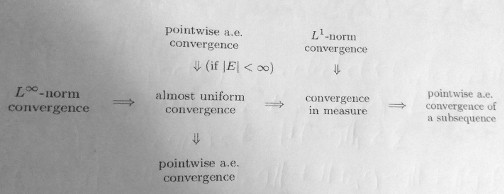
\includegraphics[width=0.85\textwidth]{images/ModesOfConvergenceRealAnalysisChart.jpg}} 
\end{center} 

\begin{prop}[Almost Everywhere Convergence of a Subsequence] 
Convergence in probability implies that there exists a 
subsequence $(k_n)$ of the original sequence which almost surely 
converges:
\[
\exists \{k_n\}_{n \geq 1} \subseteq \mathbb{N}: 
X_n \xrightarrow{\mathbb{P}} X \implies X_{k_n} \xrightarrow{a.s.} X. 
\] 
\end{prop} 
\begin{proof}[Disproof: Counterexample to Convergence in Probability Implies Almost Sure Convergence]
We will demonstrate a sequence of random variables 
that converges in probability to zero on $[0,1]$, but which does 
not converge almost surely to zero. 
For $n \geq 1$ and $1 \leq j \leq n$, define 
\[
S_{n,j} := \left[\frac{j-1}{n}, \frac{j}{n}\right] \subseteq [0,1], 
\]
and set $X_n(x) := \chi_{S_{n,j}}(x)$. Let $\varepsilon > 0$ and observe that 
\[
\PP{\{x \in [0,1] : f_n(x) > \varepsilon\}} = \PP{\{x \in [0,1] : f_n(x) = 1\}} = 
     |S_{n,j}| = \frac{1}{n} \xrightarrow[n \rightarrow \infty]{\mathbb{P}} 0. 
\] 
On the other hand, given any $x \in [0, 1]$ there are 
infinitely-many $n \in \mathbb{N}$ such that $x \in S_{n,j}$, i.e., such that 
$X_n(x) = 1$. This implies that there is a 
subsequence $\{X_{n_k}\}$ such that $X_{n_k} \xrightarrow{\mathbb{P}} 1$ and hence 
$X_n \nrightarrow 0$ almost surely on $[0,1]$. 
\end{proof}
\begin{proof}[Proof: Existence of an Almost Surely Convergent Subsequence] 
Suppose that $X_n \xrightarrow{\mathbb{P}} X$. We need to find a subsequence $\{X_{n_k}\}_{k \geq 1}$ 
such that $X_{n_k} \xrightarrow{a.s.} X$ as $k \rightarrow \infty$ for all 
$\omega \in A$ 
where $A \subseteq \Omega$ is some large enough event in the sample space such that $\PP{A} = 1$. 
For $j \geq 1$, choose $L_j$ such that for all $k \geq L_j$ 
\[
\PP{\{\omega : |X_k-X|(x) \geq 1/j\}} < \frac{1}{2^j}. 
\]
We can just as well assume here that the $L_j$'s satisfy: $L_1 < L_2 < L_3 < \cdots$. 
For $j \geq 1$, we define 
\[
E_j := \{\omega : |X_{L_j}-X|(\omega) \geq 1/j\}, 
\]
and set 
\[
Z := \limsup_{j \rightarrow \infty} E_j = \bigcap_{m \geq 1} \bigcup_{j \geq m} E_j. 
\]
Now for $m \geq 1$, we can see that 
\[
\PP{Z} \leq \PP{\bigcup_{j \geq m} E_j} \leq \sum_{j \geq m} \PP{E_j} < 
     \sum_{j \geq m} 2^{-j} = 2^{1-m} \longrightarrow 0, 
\] 
as $m \rightarrow \infty$. So we conclude that $\PP{Z} = 0$. 
Next, if $\omega \in \Omega \setminus Z$, then $\omega \notin \cup_{j \geq m} E_j$ 
for some $m \geq 1$. 
This implies that $x \notin E_j$ for all $j \geq m$. Thus 
$|X_{L_j}-X|(\omega) \leq 1/j$ for $j \geq m$, which implies that 
$\lim_{j \rightarrow \infty} X_{L_j}(\omega) = X(\omega)$ for all 
$x \in \Omega \setminus Z$. 
So it suffices to take $X_{n_j} := X_{L_j}$ so that $X_{n_k} \xrightarrow{a.s.} X$, 
or equivalently with $A := \Omega \setminus Z$ so that 
$X_{n_k}(\omega) \longrightarrow X(\omega)$ for all $\omega \in A$ where, as proved above, 
$\PP{A} = \PP{\Omega} - \PP{Z} = 1 - 0 = 1$. 
\end{proof} 

\subsection{Convergence theorems (analogs to real analysis)} 

\begin{theorem}[Lebesgue's BCT] 
Let $f_n$ be integrable $\forall n \geq 1$ such that (a) $f_n \xrightarrow{\mathbb{P}} f$; 
or (b) $f_n \xrightarrow{a.s.} f$ for some measurable function $f$. 
If $|f_n(x)| \leq g(x)$ a.e. for all $n$ 
where $g$ is integrable, then $f$ is integrable and 
\[
\lim_{n \rightarrow \infty} \int |f_n-f|d\mu = 0. 
\]
\end{theorem} 

\begin{theorem}
If $f,g$ are measurable such that $|f| \leq g$ and $g$ is integrable, then $f$ is 
integrable. 
\end{theorem} 

\begin{theorem}[Monotone convergence theorem] 
Let $\{f_k\}_{k \geq 1}$ be a sequence of measurable functions on $E$. Then 
\begin{itemize} 
\item[(1)] If $f_k \nearrow f$ a.s. on $E$ and $\exists \varphi$ integrable such that 
     $f_k \geq \varphi$ a.e. in $E$ for all $k \geq 1$, then 
     \[
     \lim_{k \rightarrow \infty} \int_E f_k = \int_E f.
     \]
\item[(2)] If $f_k \searrow f$ a.s. on $E$ and $\exists \varphi$ integrable such that 
     $f_k \leq \varphi$ $\forall k \geq 1$, then 
     \[
     \lim_{k \rightarrow \infty} \int_E f_k = \int_E f.
     \]
\end{itemize} 
\end{theorem} 

\begin{theorem}[General form of LDCT] 
Let $f_k$ be measurable for all $k \geq 1$. Suppose that 
(a) $\lim_{k \rightarrow \infty} f_k = f$ a.e. in $E$; and (b) $\exists \varphi$ integrable 
such that for all $k \geq 1$, $|f_k| \leq \varphi$ a.e. in $E$. Then 
\[
\lim_{k \rightarrow \infty} \int f_k = \int f. 
\]
\end{theorem}

\begin{lemma}[Fatou]
Suppose that $E \subseteq \mathbb{R}^n$ is measurable and let $f_k \geq 0$ be measurable for all 
$k \geq 1$. Then 
\[
\liminf_{k \rightarrow \infty} \int_E f_k \geq \int_E \left(\liminf_{k \rightarrow \infty} f_k\right). 
\]
We can obtain the same conclusion if we instead assume that the $f_k \geq \varphi$ 
for all $k \geq 1$ when $\varphi$ is integrable on $E$. 
Notice that the statement of Fatou's lemma makes no a priori assumptions on the 
convergence of the sequence $\{f_k\}_{k \geq 1}$. 
\end{lemma}

\begin{theorem}[Uniform convergence theorems]
We have the following variants of uniform convergence theorems: 
\begin{itemize} 
\item $f_n \rightarrow f$ uniformly on $[a, b]$ with $f_n$ all continuous $\implies$ 
     $f$ is continuous. 
\item If $f_n$ is differentiable on $[a,b]$ and $\lim_{n \rightarrow \infty} f_n(x_0)$ 
     exists for some $x_0 \in [a,b]$ and $f_n^{\prime}$ converge uniformly on $[a,b]$, then 
     $f_n \rightarrow f$ uniformly on $[a,b]$ and 
     $f^{\prime}(x) = \lim_{n \rightarrow \infty} f_n^{\prime}(x)$ for all $x \in [a,b]$. 
\item If $f_n$ is integrable on $[a,b]$ and $f_n \rightarrow f$ uniformly, then 
     $f$ is integrable and 
     \[
     \int_{[a,b]} f = \lim_{n \rightarrow \infty} \int_{[a,b]} f_n. 
     \]
\end{itemize} 
\end{theorem}

\subsection{Properties of the modes of convergence for random variables} 


\textbf{Fact:} If $\mu(X) < \infty$, then $L^q(\mu) \subsetneq L^p(\mu)$ for any 
$0 < p < q \leq \infty$. This can be proved by applying H\"older with the conjugate 
exponents \fbox{$p_0 := q/p$ and $q_0 := q/(q-p)$}. 

\begin{prop}[Cauchy-Schwarz and H\"older inequalities] 
Note that we assume that the functions $f,g$ are both square integrable, i.e., 
$|f|^2,|g|^2$ are both integrable. If this is the case then, 
\begin{align*} 
\int_0^1 |f| & \leq \left(\int_0^1 |f|^2\right)^{1/2} \\ 
\left\lvert \int fg\right\rvert & \leq \left(\int |f|^2\right)^{1/2} \left(\int |g|^2\right)^{1/2}. 
\end{align*} 
Note that the latter equation above is the special case of the more general cases in 
\emph{H\"older's inequality} for $\frac{1}{p}+\frac{1}{q}=1 \iff p+q=pq$ when $p=q=2$: 
\[
\left\lvert \int fg \right\rvert \leq ||f||_p \cdot ||g||_q. 
\]
\textbf{Dual (conjugate) exponents:} \fbox{If $p+q = pq$, then $p = q/(q-1)$.} 
\end{prop} 
\noindent 
Note that \emph{Minkowski's theorem} states that 
$||f+g||_p \leq ||f||_p + ||g||_p$. 
Minkowski also implies that 
\[
\left\lVert \int f \right\rVert_p \leq \int ||f||_p. 
\] 
\begin{proof}[Proof of Minkowski]
We let $p$ be arbitrary with $f,g \in L^p$ and observe that: 
\begin{align*} 
||f+g||_p^p & = \int |f+g|^p = \int |f+g|^{p-1} |f+g| \\ 
     & \leq \int |f+g|^{p-1}(|f|+|g|) d\mu,\ \text{ then we apply H\"older} \\ 
     & \leq (||f||_p+||g||_p) \left(\int |f+g|^{(p-1)\frac{p}{p-1}}\right)^{1-1/p} \\ 
     & = (||f||_p+||g||_p) \frac{||f+g||_p^p}{||f+g||_p}. 
     \qedhere
\end{align*} 
\end{proof} 
\noindent 
If $\alpha > 0$, we can obtain that 
\[
\mu\left(\{x : |f(x)| > \alpha\}\right) \leq \left(\frac{||f||_p}{\alpha}\right)^p. 
\]
Another important result which is non-trivial to prove and due to Riesz is that for 
$1 \leq q < \infty$ and $g \in L^1$:
\[
||g||_q = \sup \left\{\left\lvert\int fg \right\rvert : ||f||_p=1\right\},\ 
     \text{ where } \frac{1}{p}+\frac{1}{q} = 1. 
\]

\begin{example}[Dense Class Arguments]
\emph{Compactly supported continous functions are dense in $L^1$: 
$C_c[a,b] = L^1[a,b]$.} Other dense functions in $L^p$ are the simple (i.e., staircase) functions, 
and polynomials. If $f \in L^p$ and $C$ is \emph{dense} in $L^p$ then 
$\forall \varepsilon > 0$, $\exists g \in C$ such that $||f-g||_p < \varepsilon$. 
\end{example} 

\begin{prop}
Provided that the probability space is complete: 
\begin{itemize} 

\item If $X_n \xrightarrow{P} X$ and $X_n \xrightarrow{P} Y$, then 
     $X = Y$ almost surely. 
\item If $X_n \xrightarrow{a.s.} X$ and $X_n \xrightarrow{a.s.} Y$, then 
     $X = Y$ almost surely. 
\item If $X_n \xrightarrow{L^r} X$ and $X_n \xrightarrow{L^r} Y$, then 
     $X = Y$ almost surely. 
\item If $X_n \xrightarrow{P} X$, $Y_n \xrightarrow{P} Y$, then for any 
     $a,b \in \mathbb{R}$, $aX_n+bY_n \xrightarrow{P} aX+bY$, and 
     $X_nY_n \xrightarrow{P} XY$. 
\item If $X_n \xrightarrow{a.s.} X$, $Y_n \xrightarrow{a.s.} Y$, 
     then for any 
     $a,b \in \mathbb{R}$, $aX_n+bY_n \xrightarrow{a.s.} aX+bY$, and 
     $X_nY_n \xrightarrow{a.s.} XY$. 
\item If $X_n \xrightarrow{L^r} X$, $Y_n \xrightarrow{L^r} Y$, then for any 
     $a,b \in \mathbb{R}$, $aX_n+bY_n \xrightarrow{L^r} aX+bY$. 
\item None of the above statements are true for weak convergence in 
     distribution. 
\item Convergence in distribution to a constant implies convergence in 
     probability. 

\end{itemize} 
\end{prop} 

\newpage 
\section{Laws of large numbers} 

\subsection{The weak law of large numbers} 

\begin{example}[Key Observations]
Suppose that $(X_i)_{i \geq 1}$ have the same $L^2$ norm and that 
$E[X_i] = 0$ for all $i \geq 1$. Then:
\begin{itemize} 

\item $\operatorname{Var}\left(\frac{X_1+\cdots+X_n}{n}\right) = 
     E\left[\left\lvert \frac{X_1+\cdots+X_n}{n} \right\rvert^2 
     \right]$, which implies that 
     \[
     \operatorname{Var}\left(\frac{X_1+\cdots+X_n}{n}\right) = 
     \left\lVert \frac{X_1+\cdots+X_n}{n} \right\rVert_{L^2}^2 \leq 
     \frac{1}{n}\left(||X_1||^2+\cdots+||X_n||^2\right) = ||X_1||_{L^2}^2. 
     \]
\item If $X_1 = \cdots = X_n$, then 
     $\operatorname{Var}\left(\frac{X_1+\cdots+X_n}{n}\right) = 
     \operatorname{Var}(X_1)$. 
\item If $X_1,\ldots,X_n$ are iid, then 
\[
\operatorname{Var}\left(\frac{X_1+\cdots+X_n}{n}\right) = \frac{1}{n^2} 
     \sum_{i,j=1}^n \operatorname{Cov}(X_i, X_j) = 
     \frac{1}{n^2} \sum_{m=1}^n \operatorname{Var}(X_m) = 
     \frac{1}{n} \operatorname{Var}(X_1).
\]

\end{itemize} 
\end{example} 

\begin{theorem}[WLLN]
If $X_1,\ldots,X_n$ are iid with mean $\mu$ and variance $\sigma^2$, then 
$\bar{S}_n := \frac{X_1+\cdots+X_n}{n} \xrightarrow{P,L^2} \mu$ as 
$n \rightarrow \infty$. 
\end{theorem} 
\begin{proof} 
First, we show the statement of $L^2$ convergence. Since 
$\mu = E[\bar{S}_n]$:
\[
E[(\bar{S}_n-\mu)^2] = \operatorname{Var}(\bar{S}_n) = 
     \frac{\sigma^2}{n} \rightarrow 0, 
\]
as $n \rightarrow \infty$. So $\bar{S}_n \xrightarrow{L^2} \mu$. 
Next, for all $\varepsilon > 0$, 
\[
\mathbb{P}(|\bar{S}_n-\mu| > \varepsilon) \leq 
     \frac{E[(\bar{S}_n-\mu)^2]}{\varepsilon^2} \leq 
     \frac{\sigma^2}{n\varepsilon^2} \longrightarrow 0, 
\]
as $n \rightarrow \infty$. Hence, $\bar{S}_n \xrightarrow{P} \mu$. 
\end{proof} 

\begin{theorem}[WLLN, V2]
Suppose that $X_1,\ldots,X_n$ are iid with mean $\mu$ and 
$E[X_1^4] < \infty$. Then $\bar{S}_n \xrightarrow{L^4,a.s.} \mu$. 
\end{theorem} 
\begin{proof} 
Since we can replace $X_i$ by $Y_i := X_i - \mu$ and bound the resulting 
norm of this random variable, we can assume that $\mu = 0$. Using 
Markov, 
\[
\mathbb{P}(|\bar{S}_n| > \varepsilon) = \mathbb{P}(\bar{S}_n^4 >  
     \varepsilon^4) \leq \frac{E[\bar{S}_n^4]}{\varepsilon^4} \leq 
     \frac{C}{n^2\varepsilon^4}. 
\]
Thus $\bar{S}_n \xrightarrow{P} 0$. And by Borel-Cantelli, we have that 
$$\sum_{n \geq 1} \mathbb{P}(|\bar{S}_n| \geq \varepsilon) \leq 
 \sum_{n \geq 1} \frac{C}{n^2 \varepsilon^4} < \infty,$$ 
and so $\bar{S}_n \xrightarrow{a.s.} 0$. 
\end{proof} 

\begin{theorem} 
If $X_1,\ldots,X_n$ are independent with mean $\mu$ and are uniformly 
integrable, then $\bar{S}_n \xrightarrow{L^1,P} \mu$. 
\end{theorem}

\begin{example}[Spring 2019, \#3]
Assume that $\{X_n\}_{n \geq 1}$ are random variables such that 
\begin{itemize} 

\item[1.] $E[X_n] = 0$ and $E[X_n^2] \leq 1$ for any $n \geq 1$; 
\item[2.] $E[X_iX_j] \leq 0$ for any $i \neq j$. 

\end{itemize} 
Show that for any sequence $\{a_n\}_{n \geq 1} \subset [1/2,2]$, 
\[
\frac{a_1X_1+a_2X_2+\cdots+a_nX_n}{a_1+a_2+\cdots+a_n} 
     \xrightarrow[n \rightarrow \infty]{\mathbb{P}} 0. 
\]
\end{example} 

\subsection{Large deviations} 

If $X_1,\ldots,X_n$ are iid with mean $0$ and $E[e^{\alpha|X_1|}] < \infty$ 
for some $\alpha > 0$, then 
$$\mathbb{P}(|\bar{S}_n| > \varepsilon) \leq 2e^{-nI(\varepsilon)},$$ 
where the \textbf{\emph{rate function}} $I(\varepsilon)$ is given by 
$$I(\varepsilon) = \sup_{\lambda \in \mathbb{R}} \left\{ 
     \varepsilon\lambda - \log E[e^{\lambda X_1}]\right\}.$$ 
The function $f(\lambda) := \log E[e^{\lambda X_1}]$ is a convex function 
with 
\[
f(0) = 0, f^{\prime}(0) = E[X_1], f^{\prime\prime}(0) = 
     \frac{E[X_1^2 e^{\lambda X_1}] E[e^{\lambda X_1}] - 
     E[X_1 e^{\lambda X_1}]^2}{E[e^{\lambda X_1}]^2} \geq 0. 
\]
Also, the rate function is convex and satisfies 
\[
I(0) = 0, I^{\prime}(0) = 0, I^{\prime\prime}(0) = \frac{\sigma^2}{2} = 
     \frac{\operatorname{Var}(X_1)}{2}. 
\]
We remark that if $I(a) < \infty$, then $\bar{S}_n$ "visits" 
$(a-\varepsilon,a+\varepsilon)$ with positive probability. 

\begin{theorem} 
The \emph{moment generating function} of a random variable $X$ is 
defined to be $M(\lambda) := E[e^{\lambda X}]$. Define 
$$I(a) := \sup_{\lambda \in \mathbb{R}} \left\{a\lambda - 
     \log M(\lambda)\right\}.$$ 
Then 
\begin{itemize} 

\item[(1)] $\mathbb{P}(\bar{S}_n \geq a) \leq e^{-nI(a)}$, for $a > \mu$; 
\item[(2)] $\mathbb{P}(\bar{S}_n \leq a) \leq e^{-nI(a)}$, for $a < \mu$; 
\item[(3)] We have that 
\[
\mathbb{P}(|\bar{S}_n - a| < \varepsilon) \geq \left( 
     \frac{1-F(a)}{n\varepsilon^2}\right) e^{-n(I(a) + \varepsilon G(a))}, 
\]
where the functions $F,G$ are explicit in terms of $\mu,I,M$. 

\end{itemize} 
\end{theorem}  

\begin{theorem}[WLLN, V3]
If $(X_i)_{i \geq 1}$ are uncorrelated with mean $\mu$ such that 
$\sigma^2 = \sup_{i \geq 1} \operatorname{Var}(X_i) < \infty$, then 
$\bar{S}_n \xrightarrow{P,L^2} \mu$ as $n \rightarrow \infty$. 
\end{theorem} 

\begin{theorem}[WLLN, First Improvement, V4]
If $(X_i)_{i \geq 1}$ are iid, $\mu = E[X_i]$, and $E[X_1^4] < \infty$, 
then $\bar{S}_n \xrightarrow{P,L^4,a.s.} \mu$ as $n \rightarrow \infty$. 
\end{theorem} 
\begin{proof} 
\emph{This proof is instructive}. We assume that we have $\mu = 0$, as otherwise 
we can take $\widetilde{X}_i := X_i - \mu$ and notice that 
$||\widetilde{X}_i||_{L^4} \leq \mu + ||X_i||_{L^4} < \infty$. 
Next, we can expand 
\[
E[\bar{S}_n^4] = \frac{1}{n^4} E[(X_1+\cdots+X_n)^4] = \frac{1}{n^4} 
     \sum_{i,j,k,\ell=1}^n E[X_iX_jX_kX_{\ell}]. 
\]
Observe that if one of the indices $i,j,k,\ell$ appears by itself in the 
previous expansion, then $E[X_iX_jX_kX_{\ell}] = 0$ (by independence). 
The surviving terms are of the forms 
$(ij\hat{k}\hat{\ell}),(\hat{i}j\hat{k}\ell),(\hat{i}jk\hat{\ell})$ and 
$i=j=k=\ell$. In the first three cases, we obtain terms of 
$E[X_1^2]^2$, and in the last case we obtain $E[X_1^4]$. This implies that 
\[
E[\bar{S}_n^4] = \frac{1}{n^4}\left(3n(n-1) E[X_1^2]^2] + 
     n E[x_1^4]\right). 
\]
Now since $\operatorname{Var}(X_1^2) = E[X_1^4] - E[X_1^2]^2 \geq 0$, 
we have that 
\[
E[\bar{S}_n^4] \leq \frac{1}{n^4}(3n(n-1)+n) E[X_1^4] \leq 
     \frac{3 E[X_1^4]}{n^2}. 
\]
Then this implies that 
\[
\mathbb{P}(|\bar{S}_n| \geq \varepsilon) = \mathbb{P}(\bar{S}_n^4 \geq 
     \varepsilon^4) \leq \frac{3 E[X_1^4]}{n^2\varepsilon^4} 
     \longrightarrow 0, 
\]
as $n \rightarrow \infty$. And also, by Borel-Cantelli, we have that 
$\bar{S}_n \xrightarrow{a.s.} 0$ as $n \rightarrow \infty$. 
\end{proof} 

\begin{remark}[Observations and Extensions] 
If $(X_i)$ are independent, $E[X_i] = 0$ for all $i \geq 1$, and 
$\sup_{i \geq 1} E[X_i^4] < \infty$, then 
$\bar{S}_n \xrightarrow{P,L^4,a.s.} 0$. 
If $(X_i)_{i \geq 1}$ are independent, 
$E[X_i] = 0$ $\forall i$, and $\sup_{i \geq 1} E[X_i^{2k}] < \infty$, then 
$\bar{S}_n \xrightarrow{P,L^{2k},a.s.} 0$. In fact, we can show that 
$\mathbb{P}(|\bar{S}_n| \geq \varepsilon) \leq 
 \frac{C_k}{(n\varepsilon^2)^k}$, where the constant $C_k$ depends only on 
the fixed $k \geq 1$. 
\end{remark}

\subsection{The strong law of large numbers} 

\begin{theorem}[SLLN]
Suppose that $X_1,\ldots,X_n$ are iid. Then $\bar{S}_n \xrightarrow{a.s.} \mu$ as 
$n \rightarrow \infty$ if and only if $E[|X_1|] < \infty$ and $E[|X_1|] = \mu$. 
\end{theorem} 

\begin{remark}[Finite Expectations and Forward Direction Proof Steps]
Recall that 
\[
E[|X|] < \infty \iff \sum_{n \geq 1} \mathbb{P}[|X| > n] < \infty.
\]
This is because we know that 
\[
E[|X|] = \int_0^{\infty} \mathbb{P}[|X| \geq x] dx. 
\]
And as we can see by taking unit-width rectangles, i.e., to show that 
\[
f(1)+f(2)+\cdots \leq \int_0^{\infty} f(x) dx \leq f(0)+f(1)+f(2)+\cdots,
\]
we have that when $f$ is non-increasing (for all large enough $x \gg 1$):
\[
\int_0^{\infty} f(x) dx < \infty \iff \sum_{n \geq 1} f(n) < \infty.
\]
Now, secondly, we also observe that if 
$\frac{S_n}{n} \xrightarrow[n \rightarrow \infty]{a.s.} \mu$, then 
$\frac{X_n}{n} = \frac{S_n-S_{n-1}}{n} \xrightarrow{a.s.} 0$. To see this we 
look at the limiting behavior of 
$\frac{X_n}{n} = \frac{S_n}{n} - \left(\frac{n-1}{n}\right) \frac{S_{n-1}}{n-1} 
 \longrightarrow 0$. So we conclude that $\frac{X_n}{n} \xrightarrow{a.s.} 0$. \\ 
\textbf{Claim:} This observation implies that $X_1$ is integrable. 
\begin{proof}
Suppose that in fact $X_1$ is not integrable. Then we have that 
$\sum_{n \geq 1} \mathbb{P}[|X_1| > n] = +\infty$. So in fact since the 
$X_i$'s are independent, by Borel-Cantelli (II), 
$\mathbb{P}\left[\limsup_{n \rightarrow \infty} \{|X_n| > n\}\right] = 1$. 
But this contradicts our fact proven above that $\frac{X_n}{n} \rightarrow 0 \neq 1$. 
\end{proof} 
Finally, in summary if $E[|X_1|] < \infty$, we have proved that 
$\frac{S_n}{n} \xrightarrow{\mathbb{P}} \mu$, with $\mu = E[|X_1|]$. 
Also, though we have that $\frac{S_n}{n} \xrightarrow{a.s.} \mu_0$, so we obtain that 
in fact this $\mu_0 = E[|X_1|]$. This concludes the proof of the forward direction of the 
SLLN.
\end{remark} 

\begin{lemma}[Real Analysis Fact]
If $\sum_{n \geq 1} \frac{x_n}{n} < \infty$, then immediately 
$\frac{x_1+\cdots+x_n}{n} \rightarrow 0$. 
\end{lemma}
\begin{proof} 
By hypothesis, we have that $S_n \xrightarrow S$ as $n \rightarrow \infty$. 
Now if $S_n := \sum_{i=1}^n \frac{x_i}{i}$, then $x_n = (S_n-S_{n-1}) \cdot n$. 
So 
\begin{align*} 
\frac{x_1+\cdots+x_n}{n} & = \frac{1}{n}\left(S_1-S_0+2(S_2-S_2)+\cdots+n(S_n-S_{n-1})\right) \\ 
     & = \frac{1}{n}\left(S_0-S_1-S_2-\cdots-S_{n-1}+nS_n\right) \\ 
     & = S_n - \frac{S_0+\cdots+S_{n-1}}{n} \longrightarrow S := 0.
     \qedhere
\end{align*} 
\end{proof} 

\begin{theorem}[Kolmogorov]
If $Y_n$ is a sequence of independent random variables such that 
$\sum_{n \geq 1} \operatorname{Var}(Y_n) < \infty$, then 
$\sum_{n \geq 1} Y_n$ is a.s. convergent. 
If $Y_n := \frac{X_n}{n}$ satisfies 
$\sum_{n \geq 1} \frac{\operatorname{Var}(X_n)}{n^2} < \infty$, then 
$\sum_{n \geq 1} \frac{X_n - E[X_n]}{n} < \infty$. 
As a consequence, if $X_1,\cdots,X_n$ are iid with mean $\mu$ and finite 
variance, then $S_n \xrightarrow{a.s.} \mu$. 
\end{theorem} 

As a comment, if $\operatorname{Var}(X_1) < \infty$, we have already proved that 
\[
\mathbb{P}\left[|S_n - \mu| > \varepsilon\right] \leq 
     \frac{\operatorname{Var}(X_1)}{n \varepsilon^2}, 
\]
but in this case it's NOT Borel-Cantelli that provides the a.s. convergence. 

\begin{remark} 
To finish the sketch of the reverse direction of the SLLN, we next sketch the last 
remaining key ideas to this part of the proof. In particular, we can 1) use 
Borel-Cantelli to show the following: 
\[
\sum_{n \geq 1} \mathbb{P}[Y_n \neq X_n] = \sum_{n \geq 1} \mathbb{P}[|X_n| > n] = 
     \sum_{n \geq 1} \mathbb{P}[|X_1| > n] \implies 
     \mathbb{P}[\limsup_{n \rightarrow \infty} \{X_n \neq Y_n\}] = 0, 
\]
i.e., for all large enough $n$, $X_n = Y_n$ (a.s.) -- so that 
\[
\frac{X_1+\cdots+X_n}{n} \xrightarrow{a.s.} \mu \iff 
     \frac{Y_1+\cdots+Y_n}{n} \xrightarrow{a.s.} \mu.
\]
Then 2) we can use Kolomogorov's theorem on the variance to show that 
$\frac{Y_1+\cdots+Y_n}{n} \xrightarrow{a.s.} \mu$. 
\end{remark} 

\begin{cor}[Consequences of the SLLN] 
If $X_1,\ldots,X_n$ are iid, then for any $f: \mathbb{R} \rightarrow \mathbb{R}$ which is 
measurable and bounded, we have that 
$\sum_{i=1}^n \frac{f(X_i)}{n} \rightarrow E[f(X_i)]$. For example, suppose that 
$f(x) := \chi_{[a,b]}(x)$. Then 
$\frac{1}{n} \sum_{i=1}^n \chi_{[a,b]}(X_i) \rightarrow E[\chi_{[a,b]}(X_1)] = 
 \mathbb{P}[a \leq X_1 \leq b]$, where the former (non-limiting) sum corresponds to the 
relative frequence of $X_i$ in $[a,b]$. Now for the special case where 
$a = -\infty$ and $b = x$, we obtain that 
\[
\frac{1}{n} \sum_{i=1}^n \chi_{(-\infty,x]}(X_i) \longrightarrow F_{X_1}(x) \equiv 
     \mathbb{P}[X_1 \leq x]. 
\]
\end{cor} 

\begin{example}[Spring 2018, \#2]
Suppose that $f$ is a continuous function on $[0,1]$. Use the Law of 
Large Numbers to prove that 
\[
\lim_{n \rightarrow \infty} \int_0^1\cdots\int_0^1 
     f\left((x_1\cdots x_n)^{1/n}\right) dx_1\cdots dx_n = 
     f\left(\frac{1}{e}\right). 
\]
\end{example} 

\begin{example}[Fall 2018, \#1]
Use the SLLN to find the following limit:
\[
\lim_{n \rightarrow \infty} \int_0^1 \cdots \int_0^1 
     \frac{x_1^2+\cdots+x_n^2}{x_1+\cdots+x_n} dx_1\cdots dx_n. 
\]
\end{example} 

\begin{example}[Spring 2017, \#3]
Let $X_1,X_2,\ldots$ be iid random variables uniformly distributed on $[0,1]$. 
Show that with probability $1$, 
\[
\lim_{n \rightarrow \infty} (X_1 \cdots X_n)^{1/n}, 
\]
exists and compute its value. 
\end{example} 

\begin{example}[Spring 2015, \#8]
Let $(X_n)_{n \geq 1}$ be an iid sequence of positive random variables 
such that $E[X_1] < \infty$. Let 
\[
N_t := \sup \{n: X_1+\cdots+X_n \leq t\}. 
\]
Show that 
\[
\frac{N_t}{t} \xrightarrow[n \rightarrow \infty]{a.s.} \frac{1}{E[X_1]}, 
\]
where the convergence is in the almost sure sense. 
\end{example} 

\subsection{Concentration inequalities} 

\begin{theorem}
If $X_1,\ldots,X_n$ are iid such that $a \leq X_i \leq b$ for all $i$, then 
$$\mathbb{P}(|\bar{S}_n-\mu| > \varepsilon) \leq 
  2e^{-2n\varepsilon^2 / (b-a)^2}.$$ 
\end{theorem} 
\begin{proof}[Proof Notes]
We require the following lemma: If $a \leq X \leq b$, then 
$\operatorname{Var}(X) \leq \frac{(b-a)^2}{4}$. 
\end{proof} 

\begin{prop} 
A function $f: \mathbb{R}^n \rightarrow \mathbb{R}$ is 
\emph{$1$-Lipschitz} if 
$$|f(x_1,\ldots,x_n) - f(y_1,\ldots,y_n)| \leq 
  \sqrt{\sum_{i=1}^n (x_i-y_i)^2}.$$ 
Suppose that $X_1,\ldots,X_n$ are iid, $X_1 \sim N(0, 1)$, and that $f$ 
is $1$-Lipschitz on $\mathbb{R}^n$ such that $f$ is differentiable and 
$\sup_{x \in \mathbb{R}^n} |\nabla f(x)| \leq 1$. Then 
$$\mathbb{P}\left(|f(x_1,\ldots,x_n) - E[f(x_1,\ldots,x_n)]| > 
  \varepsilon\right) \leq e^{-\varepsilon^2 / 2}.$$ 
\end{prop} 

\begin{example}[Cauchy-Schwarz and $1$-Lipschitz Functions] 
(\textbf{\emph{Important.}}) 
An example of a $1$-Lipschitz function $f$ is given by 
$f(x_1,\ldots,x_n) := \frac{x_1+\cdots+x_n}{\sqrt{n}}$. 
To show this, we can pull a trick out of our hat in the form of 
"forcing" the Cauchy-Schwarz inequality in the following form:
\[
\left(\frac{1}{\sqrt{n}} \sum_{i=1}^n a_i\right)^2 \leq 
     \frac{1}{n} \left(\sum_{i=1}^n 1^2\right)\left(\sum_{i=1}^n 
     a_n^2\right) = \sum_{i=1}^n a_i^2. 
\]
In our case, we have that 
\[
|f(\vec{x}) - f(\vec{y})| \leq \sum_{i=1}^n |x_i-y_i| \implies 
     \frac{1}{\sqrt{n}} \sum_{i=1}^n \leq \sqrt{\sum_{i=1}^n 
     |x_i-y_i|^2}. 
\]
\end{example} 

\begin{example}
If $X_1,\ldots,X_n$ are iid with $X_1 \sim N(0, 1)$, we get that for 
$f(x_1,\ldots,x_n) := \frac{1}{\sqrt{n}}(x_1+\cdots+x_n)$:
\begin{align*} 
\mathbb{P}\left(\left\lvert \frac{1}{\sqrt{n}} \sum_i X_i - 
     E\left[\frac{1}{\sqrt{n}} \sum_i X_i\right]\right\rvert > 
     \lambda\right) & \leq 2e^{-\lambda^2/2} \\ 
\mathbb{P}\left(\left\lvert\sum_{i=1}^n X_i\right\rvert > \sqrt{n}\lambda 
     \right) & \leq 2e^{-\lambda^2/2},\ \forall \lambda > 0. 
\end{align*} 
And if we take $\lambda := \sqrt{n} \varepsilon$, then 
\[
\mathbb{P}\left(\frac{1}{n}\left\lvert \sum_{i=1}^n X_i\right\rvert > 
     \varepsilon\right) \leq 2e^{-n\varepsilon^2 / 2}. 
\]
\end{example} 

\begin{example}[Spring 2018, \#6]
Let $(X_n)_{n \geq 1}$ be a sequence of iid random variables with 
\[
\PP{X_n = 1} = \frac{1}{2} = \PP{X_n = -1}. 
\]
Let $(Y_n)_{n \geq 1}$ be a bounded sequence of random variables such that 
$\PP{Y_n \neq X_n} \leq e^{-n}$. Show that 
\[
\frac{1}{n} E[(Y_1+\cdots+Y_n)^2] \longrightarrow 1, 
\]
as $n \rightarrow \infty$. 
\end{example} 

\begin{example}[Spring 2017, \#2; Spring 2016, \#1]
Let $X$ be a random variable with mean zero and finite variance $\sigma^2$. 
Prove that for every $c > 0$, 
\[
\PP{X > c} \leq \frac{\sigma^2}{\sigma^2+c^2}. 
\]
(HINT: Combine the inequality $E[c-X] \leq E[(c-X)\chi_{X < c}]$ with the 
Cauchy-Schwarz inequality.) \\ 
(HINT: Write $c-X = (c-X)_{+} - (c-X)_{-}$ and then use Cauchy-Schwarz.) 
($\ast$) 
\end{example} 

\newpage 
\section{Normal distributions} 
\label{Section_NormalRVs} 

\subsection{One-dimensional case}

\begin{definition}[Normal and Standard Normal Distrubutions]
We say that $Z \sim N(0, 1)$ and $X \sim N(\mu, \sigma^2)$ if their 
probability density functions satisfy
\begin{align*} 
f_{Z}(x) & = \frac{1}{\sqrt{2\pi}} e^{-x^2/2},\ x \in \mathbb{R} \\ 
f_{X}(x) & = \frac{1}{\sqrt{2\pi\sigma^2}} e^{-(x-\mu)^2 / 2\sigma^2},\ 
     x \in \mathbb{R}. 
\end{align*} 
One key important fact relating these two normal distributions is that if 
$X \sim N(\mu,\sigma^2)$, then the random variable 
$Z := \frac{X-\mu}{\sigma} \sim N(0, 1)$. In particular, 
given this definition, $F_Z(z) = F_X(\sigma z+\mu)$ and 
$f_Z(z) = \sigma \cdot f_X(\sigma z+\mu)$. 
\end{definition} 

\begin{prop}[Properties of the Standard Normal]
We have the following properties of a standard normal random variable 
$Z \sim N(0, 1)$:
\begin{itemize} 

\item[(1)] $E[Z] = 0$ and $\operatorname{Var}(Z) = 1$; 
\item[(2)] $M_Z(\lambda) = E[e^{\lambda Z}] = e^{\lambda^2/2}$ for all 
     $\lambda \in \mathbb{C}$. 
     
\end{itemize} 
\end{prop} 
\begin{proof}[Proof of (1)]
First, we compute that 
\[
E[Z] = \int_{-\infty}^{\infty} z f_Z(z) dz = \int_{-\infty}^{\infty} 
     \frac{z}{\sqrt{2\pi}} e^{-z^2/2} dz = 0, 
\]
since the right-hand-side integral is of an odd function over a symmetric 
interval. Next, we can compute by repeated integration by parts that 
\begin{align*} 
\operatorname{Var}(Z) & = \frac{1}{\sqrt{2\pi}} \int_{-\infty}^{\infty} 
     z^2 e^{-z^2/2} dz \\ 
     & = \frac{1}{\sqrt{2\pi}} \int_{-\infty}^{\infty} z \left( 
     -e^{-z^2/2}\right) dz \\ 
     & = ze^{-z^2/2} \Biggr\rvert_{-\infty}^{\infty} + 
     \frac{1}{\sqrt{2\pi}} \int_{-\infty}^{\infty} e^{-z^2/2} dz \\ 
     & = 1. 
     \qedhere
\end{align*} 
\end{proof} 
\begin{proof}[Proof of (2)]
We have that 
\begin{align*} 
M_Z(\lambda) & = E[e^{\lambda Z}] = \int_{-\infty}^{\infty} 
     \frac{e^{\lambda z}}{\sqrt{2\pi}} e^{-z^2/2} dz \\ 
     & = \frac{e^{\lambda^2/2}}{\sqrt{2\pi}} \int_{-\infty}^{\infty} 
     e^{-\frac{1}{2}(z^2-2\lambda z+\lambda^2)} dz \\ 
     & = e^{\lambda^2 / 2}. 
     \qedhere 
\end{align*} 
\end{proof} 

\begin{cor}
If $X \sim N(\mu,\sigma^2)$, then its moment generating function is 
given by $M_X(\lambda) = e^{\lambda\mu+(\lambda\sigma)^2 / 2}$. 
\end{cor} 
\begin{proof} 
We can write $X = \mu + \sigma Z$, where $Z \sim N(0, 1)$. This implies 
that 
\begin{align*} 
M_X(\lambda) & = E[e^{\lambda X}] = E[e^{\lambda(\mu+\sigma Z)}] 
     = e^{\lambda\mu} E[e^{\lambda\sigma Z}] = 
     e^{\lambda\mu+\lambda^2\sigma^2 / 2}. 
     \qedhere 
\end{align*} 
\end{proof} 
Note that the moments of a normal $Z \sim N(\mu, \sigma^2)$ are given by 
\[
E[Z^n] = \begin{cases} 
     0, & \text{if $n$ is odd; } \\ 
     \sigma^n \cdot (n-1)!! = \sigma^n (n-1)(n-3)\cdots 3 \cdot 1, & \text{if $n$ is even.} 
     \end{cases} 
\]

\begin{example}[Fall 2018, \#3]
Let $(Z_n)_{n \geq 1}$ be iid standard normal random variables, and let 
$(a_n)_{n \geq 1} \subset \mathbb{R}$. Prove that 
$\sum_{n \geq 1} a_n Z_n^2 < \infty$ $\iff$ $\sum_{n \geq 1} a_n < \infty$. 
\end{example} 

\begin{example}[Spring 2016, \#6]
Let $X_1,X_2,\ldots$ be iid standard normal random variables, and for 
$x \in (-1, 1)$, set 
\[
Y := \sum_{n \geq 1} x^n X_n. 
\]
Show that the sum defining $Y$ converges and find its distribution. 
\end{example}

\subsection{Multidimensional normal distributions} 

\begin{definition} 
The random variable $Z := (Z_1,\ldots,Z_d)$ is a 
\emph{standard multidimensional normal vector} if $Z_1,\ldots,Z_d$ are 
iid with $Z_1 \sim N(0, 1)$. We write that 
$X = (X_1,\ldots,X_d) \sim N(\mu,C)$ with $\mu \in \mathbb{R}^d$ and 
covariance matrix $C$ if \footnote{
     Note that if $C \in \mathbb{C}^{d \times d}$ is symmetric, 
     $C \geq 0$, then 
     $C = UDU^T$ where $U$ is orthogonal and $D$ is a diagonal matrix of 
     eigenvalues of $C$. In particular, this shows that 
     $C^{1/2} = UD^{1/2}U^T$ in the computations from the last definitions. 
} 
\[
f_X(x_1,\ldots,x_d) = \frac{1}{\sqrt{(2\pi)^d (\det C)^{1/2}}} 
     e^{-\langle C^{-1}(x-\mu),x-\mu \rangle / 2}. 
\]
One particularly nice property relating these two types of multidimensional 
normal variables is that 
$X \sim N(\mu, C)$ $\iff$ $Z = C^{-1/2}(X-\mu) \sim N(0, \operatorname{Id})$ 
$\iff$ $X = \mu + C^{1/2} Z$ with $Z \sim N(0, \operatorname{Id})$. 
\end{definition} 

\begin{exercise}
Show that if $X = (X_1, \ldots, X_n) \sim N(\mu, C)$, then 
$C_{ij} = \operatorname{Cov}(X_i, X_j)$ and $E[X_i] = \mu_i$. 
\end{exercise} 

\begin{prop}[Properties and Transformations]
We have the following properties and transformation results relating 
multidimensional normal vectors:
\begin{itemize} 

\item[(1)] $X \sim N(\mu,C)$ $\iff$ $X = \mu+C^{1/2} Z$ where 
     $Z = (Z_1,\ldots,Z_d)$ for $Z_i$ iid and $Z_1 \sim N(0, 1)$. 
\item[(2)] If $X \sim N(\mu,C)$, $A: \mathbb{R}^d \rightarrow \mathbb{R}^m$ 
     is a linear map, then $Y := AX \sim N(A\mu, ACA^T)$. 
\item[(3)] If $X \sim N(\mu,C)$, then for any 
     $a_1,\ldots,a_d \in \mathbb{R}$, 
     $\sum_{i=1}^d a_iX_i \sim N\left(\sum_{i=1}^d a_iu_i, 
     \sum_{i,j=1}^n C_{ij}a_ia_j\right)$. 
\item[(4)] If $Z \sim N(0, \operatorname{Id})$ and $U$ is an 
     orthogonal matrix, then 
     $\widetilde{Z} := UZ \sim N(0, \operatorname{Id})$. 

\end{itemize} 
\end{prop} 
\begin{proof}[Sketch of (2)]
We first cite the following theorem: If $M_X(\lambda) = M_Y(\lambda)$ 
for all $||\lambda||_2 < \varepsilon$ ($\forall \varepsilon > 0$), then 
$X \sim Y$ have the same multidimensional distrubution. \\ 
\textbf{Step 1:} Notice that 
\[
M_X(\lambda) = E[e^{\langle \lambda, X \rangle}] = 
     E\left[e^{\sum_i \lambda_i X_i}\right]. 
\]
\textbf{Step 2:} We compute that 
\begin{align*} 
M_{AX}(\lambda) & = E\left[e^{\langle \lambda, AX \rangle_{\mathbb{R}^m}}  
     \right] = E\left[e^{\langle A^T\lambda, X \rangle_{\mathbb{R}^d}}  
     \right] \\ 
     & = e^{\langle A^T\lambda, \mu \rangle + \langle CA^T\lambda, 
     A^T\lambda \rangle} \\ 
     & = e^{\langle \lambda, A\mu \rangle + \langle ACA^T\lambda, 
     \lambda \rangle} \\ 
     & = M_{N(A\mu,ACA^T)}(\lambda). 
     \qedhere 
\end{align*} 
\end{proof} 

\begin{example}
Let $X := [X_1, X_2]^T \sim N(\mu, C)$ where $X = \mu + C^{1/2} Z$ for 
$Z \sim N(0, \operatorname{Id})$. Suppose that 
\[
C = \begin{bmatrix} \operatorname{Cov}_{X_1} & 0 \\ 
     0 & \operatorname{Cov}_{X_2} \end{bmatrix}, 
\]
where $\operatorname{Cov}_{X_1,X_2} = 0$ $\implies$ $X_1,X_2$ are normal 
and independent. Then 
\[
X = \mu + C^{1/2} \begin{bmatrix} Z_1 \\ Z_2\end{bmatrix} = \mu + 
     \begin{bmatrix} \operatorname{Cov}_{X_1}^{1/2} Z_1 \\ 
     \operatorname{Cov}_{X_2}^{1/2} Z_2 \end{bmatrix}, 
\]
so that $X_i = \mu_i \operatorname{Cov}_{X_i}^{1/2} Z_i$ are independent 
with the $Z_i$ independent. 
\end{example} 

\begin{theorem}[Concentration Inequality]
If $Z_1,\ldots,Z_d$ are iid with $Z_1 \sim N(0, 1)$, then for any 
1-Lipschitz function $f: \mathbb{R}^d \rightarrow \mathbb{R}$, we have that 
\[
\mathbb{P}\left(\left\lvert f(Z_1,\ldots,Z_d) - E[f(Z_1,\ldots,Z_d)] 
     \right\rvert\right) \leq C_1 \cdot e^{-C_2 \varepsilon^2}, 
\]
where the sharp constant is given by $C_2 = 1/2$. 
\end{theorem} 
\begin{proof}[Proof Components]
We cite \emph{Jensen's inequality} which states that for $\phi$ convex: 
$E[\phi(X)] \geq \phi(E[X])$. We also use the identity that 
$E[e^{\lambda f(Z)}] E[e^{-\lambda f(Z)}] = E[e^{\lambda(f(Z_1)-f(Z_2))}]$. 
\end{proof} 

\begin{example}[Fall 2016, \#4]
Let $(X, Y)$ be a normal vector in $\mathbb{R}^2$ with mean zero and 
covariance matrix:
\[
\Sigma = \begin{bmatrix} 5 & 1 \\ 1 & 10 \end{bmatrix}. 
\]
Find $E[X^2Y^2]$. 
\end{example} 

\begin{example}[Spring 2016, \#2]
Let $X = (X_1, X_2)$ be a Gaussian vector with zero mean and 
covariance matrix 
\[
\Sigma = \begin{bmatrix} 1 & \rho \\ \rho & 1 \end{bmatrix}, 
\]
where $|\rho| < 1$. Find a matrix $A$ such that $X = AZ$ where $Z$ is 
a standard normal vector, and derive the characteristic function of $X$ 
as a function of $\rho$. 
\end{example} 

\begin{example}[Spring 2015, \#3]
Assume that $(X, Y)$ is a joint normal vector with $E[X] = E[Y] = 0$. 
Show that 
\[
E[X^2Y^2] \geq E[X^2]E[Y^2], 
\]
with equality if and only if $X,Y$ are independent. 
\end{example}

\begin{remark}[Notes on the Examples] 
If we assume that $(X, Y)$ is a joint normal vector with mean $E[X]=E[Y]=0$ 
and variance $\sigma^2$, then the covariance matrix for the pair can be 
written as 
\[
C = \begin{bmatrix} \sigma^2 & \rho \\ \rho & \sigma^2 \end{bmatrix}. 
\]
This implies a formula for the characteristic function of $(X,Y)$ given by 
\[
f_{X,Y}(\xi,\eta) = E[e^{\imath \xi X + \imath \eta Y}] = 
     \exp\left(-\frac{(\xi \sigma)^2 + (\eta \sigma)^2 + 2 \rho\xi\eta}{2} 
     \right). 
\]
One usage of this characteristic function would be to compute the 
expectations 
\[
E[X^2Y^2] = \frac{1}{\imath^4} \frac{d^4}{d\xi^2 d\eta^2} f_{X,Y}(\xi,\eta) 
     \Biggr\rvert_{\xi=\eta=0}. 
\]
\end{remark} 

\newpage 
\section{Central limit theorem} 

\begin{theorem}[Central Limit Theorem]
Let $X_1,\ldots,X_n,\ldots$ be independent iid random variables with 
mean $\mu$ and finite variance. If $-\infty < a < b < \infty$, then 
\[
\lim_{n \rightarrow \infty} \mathbb{P}\left( 
     a \leq \frac{X_1+\cdots+X_n - n\mu}{\sigma\sqrt{n}} \leq b\right) = 
     \int_a^b \frac{1}{\sqrt{2\pi}} e^{-x^2 / 2} dx. 
\]
\end{theorem} 

\begin{example}[Spring 2018, \#4]
Let $X_1,\ldots,X_n$ be iid random variables with mean $\mu$ and 
variance $\sigma^2 < \infty$. Let $f$ be a function continuously 
differentiable at the point $\mu$. Prove that the sequence of random 
variables 
\[
\sqrt{n}\left(f\left(\frac{X_1+\cdots+X_n}{n}\right) - f(\mu)\right), 
\]
converges in distribution to a normal random variable. What is the 
mean and the variance of the limit? 
(HINT: Use the first-degree Taylor approximation of $f$ about $\mu$.)
\end{example} 
\begin{proof}
If we define $Y_n := \sqrt{n}\left(\frac{X_1+\cdots+X_n}{n} - \mu\right)$, 
then $Y_n \xrightarrow{\operatorname{dist}} Y$, where 
$Y \sim N(0, \sigma^2)$ (by the Central Limit Theorem). 
Also, by the SLLN $Y_n / \sqrt{n} \xrightarrow{\mathbb{P}} 0$. 
\end{proof} 

\begin{example}[Spring 2018, \#5]
Let $X_1,\ldots,X_n,\ldots$ be iid random variables with $E[X_1] = 0$ and 
$\operatorname{Var}(X_1) = 1$. Define $S_n := X_1+\cdots+X_n$. 
Prove that 
\[
\limsup_{n \rightarrow \infty} \frac{S_n}{\sqrt{n}} = +\infty. 
\]
\end{example} 

\begin{example}[Spring 2017, \#6]
Let $(X_i)$ be iid random variables which are uniformly distributed on 
$[0,2]$. Let $S_n := X_1+\cdots+X_n$. Show that 
\[
\frac{3\sqrt{3}}{2} n^{1/6}\left(\sqrt[3]{S_n} - \sqrt[3]{n}\right) 
     \implies^{w} Z, 
\]
where $Z$ is a standard normal random variable.  
\end{example} 

\begin{example}[Spring 2016, \#7]
Let $X_1,X_2,\ldots$ be independent random variables such that 
$X_n \sim \operatorname{Bernoulli}(p_n)$ for some $p_n > 0$. Show that if 
$np_n(1-p_n) \rightarrow \infty$, then 
\[
\frac{X_n - np_n}{\sqrt{np_n(1-p_n)}} \implies^{w} N(0, 1). 
\]
\end{example} 

\begin{example}[Spring 2015, \#2]
Assume that $X_1,X_2,\ldots$ is a sequence of iid random variables such 
that for some $\alpha < 1/2$,
\[
\frac{X_1+\cdots+X_n}{n^{\alpha}} \xrightarrow[n \rightarrow \infty]{a.s.} m, 
\]
for some real number $m$. Show that almost surely $X_i = 0$. 
\end{example} 


\newpage
\section{Fall 2018 Probability I final exam solutions} 

\subsection{Problem 1}

\begin{problem}
Show that a random variable $X$ such that 
\[
E[e^{\lambda X}] \leq e^{2|\lambda|^3},\ \forall \lambda \in [-1, 1], 
\]
satisfies $X = 0$ almost surely. 
\end{problem}
\begin{proof} 
First, we compute that 
\begin{align*} 
E[X] & = \lim_{\lambda \rightarrow 0} \frac{E[e^{\lambda X}] - 1}{\lambda} 
     \leq \lim_{\lambda \rightarrow 0} \frac{e^{2|\lambda|^3} - 1}{\lambda} 
     = \lim_{\lambda \rightarrow 0} \sum_{k=1}^{\infty} 
     2^k \frac{|\lambda|^{3k}}{\lambda} 
     \leq 0. 
\end{align*} 
Also, we can see by a related computation that 
\[
E[-X] = \lim_{\lambda \rightarrow 0} \frac{E[e^{-\lambda X}] - 1}{\lambda}
     \leq 0. 
\]
Thus, we conclude that $E[X] = 0$. 
Similarly, we have that 
\[
E[X^2] = \lim_{\lambda \rightarrow 0} \frac{E[e^{\lambda X}] - \lambda E[X] -1}{
     \lambda} \leq 0 \implies E[X^2] = 0, 
\]
since $E[X^2] \geq 0$. Now since $X^2 \geq 0$, we also have that 
\[
E[X^2] = \int_0^{\infty} \PP{X^2 > t} dt. 
\]
And since $E[X^2] = 0$ by the above, we must have that $\PP{X^2 > t} = 0$ a.e. 
for $t \in \mathbb{R}_{\geq 0}$. Hence, for positive $\varepsilon > 0$, 
the set of $A \subset \Omega$ such that 
$\PP{\{\omega \in A: X(\omega) > \varepsilon\}} = 0$ has full measure. 
In other words, $X = 0$ almost surely. 
\end{proof} 

\subsection{Problem 2}

\begin{problem}
Give an example of random variables $X_n$ which converge to $0$ almost 
surely, but such that $\sum_{n \geq 1} \PP{|X_n| \geq \varepsilon} = \infty$, 
for any $\varepsilon > 0$. 
\end{problem}
\begin{proof}[Solution] 
Let $\Omega := [0, 1]$. 
For $n \geq 1$, let $U \sim \operatorname{Uniform}(0,1)$ and 
define the composite random variables by 
$X_n := n \cdot \chi_{0 \leq U \leq \frac{1}{n}}$. Then for any 
$\omega \in \Omega$, 
\[
\PP{X_n(\omega) \neq 0} = \PP{\omega \in [0, 1/n]} = \frac{1}{n} 
     \longrightarrow 0, 
\]
as $n \rightarrow \infty$. For any $\varepsilon > 0$, we can also estimate 
\[
\PP{|X_n| > \varepsilon} = 
     \int_0^{\min(\varepsilon, 1/n)} \frac{1}{1/n-0} dt = 
     n \min(\varepsilon, 1/n) \implies 
     \sum_{n \geq 1} \PP{|X_n| > \varepsilon} = +\infty. 
     \qedhere
\]
\end{proof} 

\subsection{Problem 3}

\begin{problem}
The moment generating function of a random variable $X$ is defined to be 
$M_X(\lambda) = E[e^{\lambda X}]$, which may only be convergent for some 
$\lambda \in \mathbb{R}$. Prove the following: 
\begin{itemize} 

\item[a.] If $M_X(\lambda)$ is defined for some $0 < |\lambda| < \delta$,
     then 
     \[
     \PP{|X| \geq x} \leq e^{-cx}\left(M_X(c)+M_X(-c)\right), 
     \]
     for any $x > 0$ and $\delta > c > 0$; 
\item[b.] Show that if for a given random variable $X$ there exist constants 
     $c,C > 0$ such that $\PP{|X| \geq x} \leq C e^{-cx}$ for any $x > 0$, 
     then $E[e^{\lambda X}] < \infty$ for small $|\lambda| < c$; 
\item[c.] If $M_X(\lambda)$ exists for $\lambda < \delta$, with $\delta > 0$, 
     then for all $\alpha > 0$, $E[|X|^{\alpha}] < \infty$. Justify that 
     \[
     M_X(\lambda) = \sum_{k \geq 0} \frac{E[X^k] \lambda^k}{k!}. 
     \]
     We also have that 
     \[
     \frac{d^{(k)}}{d\lambda^{(k)}} M_X(\lambda) \Bigr\rvert_{\lambda = 0} = 
          E[X^k]. 
     \]

\end{itemize} 
\end{problem} 
\begin{proof}[Proof of (a)]
We start from the right-hand-side upper inequality and bound: 
\begin{align*} 
e^{-cx}\left(M_X(c) + M_X(-c)\right) & = e^{-cx} I_c + e^{-cx} 
     \int_1^{\infty}\left(\PP{X \geq \frac{\log y}{c}} + 
     \PP{-X \geq \frac{\log y}{c}}\right) dy \\ 
     & \geq c e^{-cx} \int_0^{\infty} \PP{|X| \geq t} e^{ct} dt \\ 
     & = c \int_0^{\infty} e^{c(t-x)} \PP{|X| \geq t} dt. 
\end{align*} 
We can integrate by parts with $u = \PP{|X| \geq t}$, 
$du = -f_{|X|}(t) dt$, $dv = c e^{c(t-x)} dt$, and $v = e^{-c(x-t)}$. 
This yields that 
\begin{align*} 
e^{-cx}\left(M_X(c) + M_X(-c)\right) & \geq 
     \PP{|X| \geq x} - e^{-cx} + \int_0^{\infty} e^{-cx} \chi_{[0,x]}(t) 
     e^{ct} f_{|X|}(t) dt \\ 
     & \phantom{==\ } + 
     \int_x^{\infty} c e^{-cx} \PP{|X| \geq t} e^{ct} dt \\ 
     & = 
     \PP{|X| \geq x} -e^{-cx} + E[e^{c|X|} \chi_{[0,x]}] + 
     \int_x^{\infty} c e^{-cx} \PP{|X| \geq t} e^{ct} dt. 
\end{align*} 
Now we use a special trick which we observe in the form of 
\[
E[e^{c |X|}] = 1 + c \int_0^{\infty} e^{cx} \PP{|X| \geq x} dx. 
\]
This implies that 
\begin{align*} 
e^{-cx}\left(M_X(c) + M_X(-c)\right) & \geq 
     \PP{|X| \geq x} + E[e^{c|X|} \chi_{[0,x]}] + 
     E[e^{c|X|} \chi_{(x,\infty)}] \\ 
     & = \PP{|X| \geq x} + E[e^{c|X|}] \\ 
     & \geq \PP{|X| \geq x}. 
     \qedhere
\end{align*} 
\end{proof} 
\begin{proof}[Proof of (b)] 
This proof follows almost immediately if you notice the formula in the 
first line of the next equations:
\begin{align*} 
E[e^{\lambda |X|}] & = 1 + \lambda \int_0^{\infty} e^{\lambda x} 
     \PP{|X| \geq x} dx \\ 
     & \leq 1 + \lambda C \int_0^{\infty} e^{(\lambda-c)x} dx \\ 
     & = 1 + \frac{\lambda C e^{(\lambda-c)x}}{\lambda - c} 
     \Biggr\rvert_{x=0}^{x=\infty} < \infty, 
\end{align*} 
where we get convergence of the exponential function at the limits 
since $\lambda < c$. 
\end{proof} 
\begin{proof}[Proof of (c)] 
We begin by expanding:
\begin{align*} 
\infty & > M_X(\lambda) = \int_{-\infty}^{\infty} e^{\lambda t} f_X(t) dt \\ 
     & = \int_0^{\infty} e^{\lambda |t|} f_X(t) dt \\ 
     & = \int_0^{\infty} \sum_{k=0}^{\infty} \frac{\lambda^k |t|^k}{k!} 
     f_X(t) dt \\ 
     & = \int_0^{\infty} \lim_{n \rightarrow \infty} \sum_{k=0}^n 
     \frac{\lambda^k |t|^k}{k!} f_X(t) dt. 
\end{align*} 
Since the exponential function $e^{\lambda |t|}$ is integrable, by the 
BCT (\emph{Bounded Convergence Theorem}), we have that 
\[
\tag{$\ast$} 
M_X(\lambda) = \sum_{k \geq 0} \int_0^{\infty} \frac{\lambda^k |t|^k}{k!} 
     f_X(t) dt. 
\]
Furthermore, since all of the integrands in the previous equation are 
non-negative, each integral $E[|X|^k] = \int_0^{\infty} |t|^k f_X(t) dt$ 
exists (converges). Thus we have that 
\[
M_X(\lambda) = \sum_{k \geq 0} \frac{E[X^k] \lambda^k}{k!}. 
\]
Finally, from ($\ast$) we can see that 
\[
\frac{d^{(j)}}{d\lambda^{(j)}}[M_X(\lambda)] \Biggr\rvert_{\lambda=0} = 
     \sum_{k=j}^{\infty} \frac{k!}{(k-j)!} \frac{\lambda^{k-j} E[X^k]}{k!} 
     \Biggr\rvert_{\lambda=0} = E[X^j].
     \qedhere
\]
\end{proof} 

\subsection{Problem 4}

\begin{problem}
Consider and prove each of the statements below:
\begin{itemize} 

\item[(a)] Assume $X,Y$ are two bounded random variables. If for any integer 
     numbers $m,n \geq 0$, we have 
     \[
     E[X^mY^n] = E[X^m] E[Y^n], 
     \]
     show that $X,Y$ must be independent. 
\item[(b)] Take random variables $X,Y$ such that for some 
     constant $c > 0$, we have that 
     \[
     \PP{|X| \geq x} + \PP{|Y| \geq x} \leq e^{-cx},\ \forall x > 0. 
     \]
     Precisely, we need to show that for any integers $m,n \geq 0$, 
     $X^mY^n$ is integrable. Moreover, we show that if for any such 
     $m,n \geq 0$, 
     \[
     E[X^mY^n] = E[X^m] E[Y^n], 
     \]
     then $X,Y$ are necessarily independent. 
\item[(c)] Assume that $X,Y$ are independent random variables such that 
     their moment generating functions, $M_X(\alpha) = E[e^{\alpha X}]$ and 
     $M_Y(\beta) = E[e^{\beta Y}]$, are finite for all 
     $0 < |\alpha|,|\beta| < \delta$. Prove that if 
     \[
     E[e^{\alpha X+\beta Y}] = E[e^{\alpha X}] E[e^{\beta Y}], 
          \forall |\alpha|,|\beta| < \delta, 
     \]
     then $X,Y$ must be independent. 

\end{itemize} 
\end{problem} 
%\begin{proof}[Proof of (a)] 
%\end{proof} 
\begin{proof}[Proof of (b)] 
We first assume that $X,Y$ are independent for the first part of the proof. 
Notice that by trading expansions with inclusion-exclusion, we have that 
for any $x > 0$:
\begin{align*} 
e^{-cx} & \geq \PP{|X| \geq x} + \PP{|Y| \geq x} \\ 
     & = \PP{|X| \geq x \vee |Y| \geq x} - 
     \PP{|X|^m \geq x^m} \PP{|Y|^n \geq x^m} \\ 
     & \geq \PP{|X| \geq x \vee |Y| \geq x} - 
     \frac{E[|X|^m] E[|Y|^n]}{x^{m+n}} \\ 
     & = 1 - \PP{|X| \leq x \wedge |Y| \leq x} - 
     \frac{E[|X|^m] E[|Y|^n]}{x^{m+n}} \\ 
     & = \PP{|X|^m |Y|^n \geq x^{m+n}} - 
     \frac{E[|X|^m] E[|Y|^n]}{x^{m+n}}. 
\end{align*} 
Now, $X^mY^n$ is integrable whenever its expectation is finite. So it 
suffices to show that 
\begin{align*} 
\int_1^{\infty} \PP{X^mY^n \geq t^{m+n}} dt & \leq 
     \int_1^{\infty} e^{-cx} dx 
     + E[|X|^m] E[|Y|^n] \int_1^{\infty} \frac{dx}{x^{m+n}} \\ 
     & = \frac{1}{c} e^{-c} - \frac{E[|X|^m] E[|Y|^n]}{(m+n-1)} < \infty. 
\end{align*} 
For the second statement, notice that the conclusion is trivial if 
$m=0$ or $n = 0$ since $E[1] = 1$. Thus we prove the following lemma 
for integral powers $m,n \geq 1$: \\ 
\noindent 
\textbf{Lemma:} 
Two random variables $X,Y$ are independent if and only if $X^m,Y^n$ are 
independent for all natural numbers $m,n \geq 1$. 
\begin{proof} 
Suppose that we have 
\begin{align*} 
\PP{X^m \geq x_1 \wedge Y^n \geq x_2} & = 
     \PP{X \geq x_1^{1/m} \wedge Y \geq x_2^{1/n}} \\ 
     & = \PP{X \geq x_1^{1/m}} \PP{Y \geq x_2^{1/n}} \\ 
     & \iff X,Y \text{ are independent. } 
     \qedhere
\end{align*} 
\end{proof} 
\end{proof} 
%\begin{proof}[Proof of (c)]
%\end{proof} 

\subsection{Problem 5}

\begin{problem}
For a sequence $(X_n)_{n \geq 1}$ of exponential random variables, say with 
$X_i \sim \operatorname{Exp}(\lambda_i)$ for $\lambda_i > 0$ 
$\forall i \geq 1$, find sequences of constants $a_n,b_n,c_n,d_n$ such that 
the two sequences 
\begin{align*} 
Y_n & := a_n \max(X_1,\ldots,X_n) + b_n \\ 
Z_n & := c_n \min(X_1,\ldots,X_n) + d_n, 
\end{align*} 
both converge (weakly) to some limiting distribution. Identify the 
limiting distributions. 
\end{problem} 
\begin{proof}[Solution for the Min-Variable Case]
Notice that by independence, we must have the product 
\begin{align*} 
\PP{\min(X_1,\ldots,X_n) > \frac{y-d_n}{c_n}} & = 
     \PP{X_i  > \frac{y-d_n}{c_n},\ \forall 1 \leq i \leq n} \\ 
     & = \prod_{i=1}^n \PP{X_i > \frac{y-d_n}{c_n}} = 
     \prod_{i=1}^n \exp\left[-\lambda_i\left(\frac{y-d_n}{c_n}\right) 
     \right] \\ 
     & = e^{\frac{d_n}{c_n}(\lambda_1+\cdots+\lambda_n)} \times 
     \exp\left[-y \frac{(\lambda_1+\cdots+\lambda_n)}{c_n}\right], 
\end{align*} 
which means that $\frac{1}{c_n}(Z_n-d_n)$ is a multiple of an 
exponentially distributed random variable with parameter given by 
$\frac{(\lambda_1+\cdots+\lambda_n)}{c_n}$. Now to remove the inconvenient 
multiple, and to simplify the problem, we might as well set the two 
sequences to be constant as $(c_n, d_n) := (1, 0)$ for all $n \geq 1$. 
Then if we further make the restriction that for 
\[
\lambda := \sum_{i \geq 1} \lambda_i,\ 0 < \lambda < \infty, 
\]
we obtain a limiting distribution for $Z_n$ which is exponential with 
parameter $\lambda$. 
\end{proof} 
\begin{proof}[Solution for the Max-Variable Case]
For the purposes of simplicity, we assume that all of the parameters 
$\lambda_i = \lambda$ are identical here (otherwise for the observations 
part of the question, the limiting distribution gets extremely hairly). 
For this exploratory analysis, we will use independence coupled with an 
application of inclusion-exclusion (binomial theorem) to find that 
\begin{align*} 
\PP{\max(X_1,\ldots,X_n) > \frac{y-b_n}{a_n}} & = 
     \PP{X_1 > \frac{y-b_n}{a_n} \vee \cdots \vee X_n > \frac{y-b_n}{a_n}} \\ 
     & = \sum_{k=1}^n \binom{n}{k} (-1)^{k-1} 
     \PP{X_1 > \frac{y-b_n}{a_n}}^{k} \\ 
     & = 1 - \left(1-e^{-\lambda \left(\frac{y-b_n}{a_n}\right)}\right)^{n}. 
\end{align*} 
Now let's set $a_n \equiv 1$ and declare that $b_n = \log(1/n)$, i.e., so 
that we get an exponential function in the limiting case of the last 
equation:
\begin{align*} 
\PP{\max(X_1,\ldots,X_n) > \frac{y-b_n}{a_n}} & = 
1-\left(1-\frac{e^{-\lambda y}}{n^{\lambda}}\right)^{n} \longrightarrow 
     1 - \exp\left[-\frac{1}{\lambda} e^{-\lambda y}\right]. 
\end{align*} 
Now by fiddling with the probability equations for the cumulative 
density, we can find that 
\[
\PP{\frac{1}{\lambda} \log(1 / Y_n) \geq y} 
     \xrightarrow[n \rightarrow \infty]{w} e^{-y / \lambda}. 
\]
So in summary, the sequence of random variables defined by 
$\log(Y_n^{-1/\lambda}) \rightarrow \operatorname{Exp}(1/\lambda)$ 
tend to an exponentially distributed limit as $n \rightarrow \infty$. 
\end{proof} 

\subsection{Problem 6}

\begin{problem}
Assume that $(X_n)_{n \geq 1}$ are iid with $X_1 \sim N(0, 1)$. Show that 
for any $\lambda > 1/2$, 
\[
\bar{S}_n := 
     \frac{1}{n^{\lambda}} \sum_{i=1}^n X_i 
     \xrightarrow[n \rightarrow \infty]{a.s.} 0. 
\]
\end{problem} 
\begin{proof} 
The partial sums $S_n := X_1+\cdots+X_n$ satisfy $S_n \sim N(0, n)$, with 
corresponding distribution function 
$f_{S_n}(x) = \frac{1}{\sqrt{2\pi n}} e^{-x^2 / 2n}$. Now let 
$\varepsilon > 0$ and consider the convergence of the sums 
\[
\sum_{n \geq 1} \PP{\frac{|S_n|}{n^{\lambda}} > \varepsilon} < \infty 
     \iff I_{\varepsilon} := 
     \int_1^{\infty} \PP{|S_t| > t^{\lambda} \varepsilon} dt < \infty. 
\]
With the change of variables $s = x / \sqrt{2t}$ and 
$\sqrt{2t} \cdot ds = dx$, we can re-write the last integral as the 
double integral:
\[
I_{\varepsilon} = \int_1^{\infty} \int_0^{\varepsilon t^{\lambda}} 
     \frac{1}{\sqrt{\pi}} e^{-s^2} ds dt. 
\]
Since the density function $f_{S_t}(x)$ is non-negative, continuous (hence 
measurable) and integrable on $[0, \infty)$, Fubini-Tonelli tells us that 
we can swap the order of integration in the last equation where we also 
use that $\lambda > 1/2 \implies \frac{1}{\lambda} < 2$:
\begin{align*} 
I_{\varepsilon} & = \int_1^{\infty} \int_0^{\infty} 
     \frac{e^{-s^2}}{\sqrt{\pi}} \chi_{[0,\varepsilon t^{\lambda}]}(s) 
     ds dt \\ 
     & = \int_0^{\infty} \int_{\varepsilon}^{(s / \varepsilon)^{1/\lambda}} 
     \frac{e^{-s^2}}{\sqrt{\pi}} dt ds \\ 
     & = \int_0^{\infty} \frac{e^{-s^2}}{\sqrt{\pi}} \left[ 
     \left(\frac{s}{\varepsilon}\right)^{1/\lambda} - 
     \varepsilon\right] ds \\ 
     & \leq \int_0^{\infty} \frac{s^2 e^{-s^2}}{\sqrt{\pi} 
     \varepsilon^{1/\lambda}} - \frac{\varepsilon}{2} \\ 
     & = \frac{1}{4 \varepsilon^{1/\lambda}} - \frac{\varepsilon}{2} < 
     \infty. 
\end{align*} 
So we obtain convergence of the infinite sum we wished to bound above. And 
then by Borel-Cantelli, we have that 
\[
\PP{\limsup_{n \rightarrow \infty} \{|S_n| n^{-\lambda} > \varepsilon\}} = 0, 
\]
which as we have argued before implies almost sure convergence of 
$S_n / n^{\lambda}$ to zero as $n \rightarrow \infty$. 
\end{proof} 

\begin{proof}[Note: Alternate Simple Proof]
For $S_n := X_1+X_2+\cdots+X_n$, we can also use the large deviation bound 
which provides that 
\[
\PP{|S_n| > \varepsilon} \leq 2e^{-\varepsilon^2 / 2n}, 
\]
for $\varepsilon > 0$. 
\end{proof} 

\subsection{Problem 7}

\begin{problem}
Show that for any sequence $(X_n)_{n \geq 1}$ of iid random variables, 
\[
\frac{1}{n^2} \sum_{i=1}^n i X_i \xrightarrow[n \rightarrow \infty]{a.s.} 
     \frac{m}{2} \iff X_1 \text{ is integrable and } E[X_1] = m. 
\]
\end{problem} 
\begin{proof} 
Let $R_n := X_1 + 2X_2+\cdots+nX_n$ and $S_n := X_1+\cdots+X_n$ as usual. 
We start by summing $R_n$ by parts as 
\begin{align*} 
\frac{R_n}{n^2} & = \frac{1}{n^2}\left(n S_n - \sum_{k=1}^{n-1} S_k\right) \\ 
     & = \frac{1}{n^2}\left(n S_n - (n-1)X_1 - (n-2) X_2 - \cdots - 
     2 X_{n-2} - X_{n-1}\right) \\ 
     & = \bar{S}_n - \sum_{k=1}^{n-1} \left(\frac{1}{n} - \frac{k}{n^2} 
     \right) X_k \\ 
     & = \bar{S}_n - \frac{(n-1)}{n} \bar{S}_{n-1} + 
     \frac{(n-1)^2}{n^2} \frac{R_{n-1}}{(n-1)^2}. 
\end{align*} 
Let $m > n \geq 1$ be integers. We can show that the sequence 
$R_n / n^2$ is Cauchy, i.e., that its limit exists (call it $\widetilde{R}$): 
\begin{align*} 
\left\lvert\frac{R_n}{n^2} - \frac{R_m}{m^2}\right\rvert & \leq 
     |\bar{S}_n - (1-1/n) \bar{S}_{n-1}| + |\bar{S}_m - (1-1/m) \bar{S}_{m-1}| \\ 
     & \phantom{==\ } + 
     (1+o(1))\left\lvert \left(\frac{1}{(n-1)^2}-\frac{1}{(m-1)^2}\right) 
     R_{n-1} - \sum_{k=n}^{m-1} \frac{kX_k}{(m-1)^2}\right\rvert \\ 
     & \rightarrow \left\lvert \sum_{k=n}^{m-1} \frac{kX_k}{(m-1)^2} 
     \right\rvert 
     \leq \left\lvert \frac{S_{m-1} - S_{n-1}}{m-1}\right\rvert \\ 
     & = \left\lvert \bar{S}_{m-1} - \left(1-\frac{(m-n)}{m-1}\right) 
     \bar{S}_{n-1}\right\rvert \\ 
     & \rightarrow 0, 
\end{align*} 
as $m \rightarrow \infty$ and then $n \rightarrow \infty$. 
Now, by a rearrangement of the last expressions for $R_n$, we can write 
\[
R_n = (n-1) S_n - X_n - R_n + n \cdot X_n. 
\]
Thus by the SLLN we have that $X_1$ is integrable and $E[X_1] = m$ $\iff$ 
\[
\frac{2R_n}{n^2} \xrightarrow[n \rightarrow \infty]{a.s.} \lim_{n \rightarrow \infty} \left[ 
    \frac{(n-1)}{n} \bar{S}_n - \frac{X_n}{n^2} + \frac{X_n}{n}\right] = m. 
\]
This implies the claimed result. 
\end{proof} 

\subsection{Problem 8}

\begin{problem}
Show that for a sequence of symmetric random variables $X_2,X_2,\ldots$ 
with finite moment generating function, and 
$S_n := \frac{2}{n(n+1)} \sum_{i=1}^n iX_i$, then 
\[
\PP{|S_n| \geq x} \leq 2 \exp\left(-(n+1) I\left(\frac{nx}{n+1}\right)\right), 
\]
where 
\[
I(x) = \sup_{\lambda \in \mathbb{R}} \left\{\frac{x\lambda}{2} - 
     \int_0^1 \Lambda(\lambda t) dt\right\}, 
\]
where $\Lambda(\lambda) = \log M(\lambda)$ and 
$M(\lambda) = E[e^{\lambda X_1}]$. NOTE: Here, by a symmetric random variable 
$X$ we mean that $X$ and $-X$ have the same distributions.
\end{problem}
\begin{proof}
Given the symmetry of the variables, we only need to show the inequality for 
one side. Namely, it suffices to show that for $x \geq 0$, 
\[
\PP{S_n \geq x} \leq \exp\left(-(n+1) I\left(\frac{nx}{n+1}\right)\right). 
\]
We proceed using the standard tool for \emph{Large Deviations} by writing 
\begin{align*} 
\PP{S_n \geq x} & = \PP{e^{n\lambda S_n/2} \geq e^{n\lambda x/2}} \leq 
     \frac{E[e^{n\lambda S_n}]}{e^{n\lambda x}} \\ 
     & = \exp\left(-\frac{n\lambda x}{2} + \sum_{k=1}^n 
     \log E[e^{k\lambda X_1 / (n+1)}]\right) \\ 
     & = \exp\left(-n\left\{\frac{\lambda x}{2} - \frac{1}{n} 
     \sum_{k=1}^n \Lambda(k\lambda / (n+1))\right\}\right). 
\end{align*} 
The key now is to show our claim that 
\[
\tag{$\ast$} 
\sum_{k=1}^n \Lambda(k\lambda / (n+1)) \leq (n+1) \int_0^1 \Lambda(t\lambda) dt. 
\]
To this end, notice that because $X_1$ is symmetric, we will show that 
$\Lambda$ is non-decreasing as a function of $\lambda \geq 0$. Indeed, 
\[
\Lambda^{\prime}(\lambda) = \frac{E[X e^{\lambda X}]}{E[e^{\lambda X}]}. 
\]
Now, from the symmetry of $X$, we have that 
\[
E[Xe^{\lambda X}] = \frac{1}{2}\left(E[Xe^{\lambda X}] + 
     E[(-X)e^{\lambda(-X)}]\right) = E[X \sinh(\lambda X)], 
\]
where $\sinh(x) = (e^x-e^{-x}) / 2$. 
Since $\lambda > 0$, is is easy to see that $X \sinh(\lambda X) \geq 0$. 
Thus we conclude that $\Lambda$ is non-decreasing on $[0, \infty)$. In 
addition, $\Lambda(\lambda) \geq 0$ for any $\lambda \geq 0$. 

Using these observations, we show the claim in ($\ast$) using that for 
each time interval $[k/(n+1),(k+1)/(n+1)]$ with $k = 0,1,2,\ldots,n$ that 
\[
\Lambda(k\lambda / n) \leq (n+1) \int_{k/(n+1)}^{(k+1)/(n+1)} 
     \Lambda(t\lambda) dt. 
\]
Summing over these time intervals we obtain ($\ast$) -- and in particular, 
we also get that 
\[
     \PP{S_n \geq x} \leq \exp\left(-n\left\{\frac{\lambda x}{2} - 
     \frac{n+1}{n} \int_0^1 \Lambda(\lambda t) dt\right\}\right) = 
     \exp\left(-(n+1) I\left(\frac{nx}{n+1}\right)\right). 
     \qedhere 
\]
\end{proof}

\subsection{Problem 9}

\begin{problem}
Find the rate function of the large deviation of a sequence of iid 
random variables with Poisson distribution with parameter $a < 0$. 
\end{problem} 
\begin{proof}[Solution]
If the $X_n \sim \operatorname{Poisson}(a > 0)$, then for natural numbers $k \geq 0$, we have that 
\[
\mathbb{P}[X_n = k] = e^{-a} \frac{a^k}{k!}. 
\]
Since the sequence is iid, it suffices to find the rate function corresponding to $X_1$, 
which is defined to be 
\[
I(\varepsilon) = \sup_{\lambda \in \mathbb{R}} \left\{\varepsilon\lambda - 
     \log E[e^{\lambda X_1}] \right\}. 
\]
Here, we have that the discrete expectation is defined by 
\begin{align*} 
E[e^{\lambda X_1}] & = \sum_{k \geq 0} e^{\lambda k} \mathbb{P}[X_1 = k] \\ 
     & = \sum_{k \geq 0} \frac{(e^{\lambda} a)^k}{k!} \\ 
     & = e^{a(e^{\lambda}-1)} \\ 
     & \implies \log E[e^{\lambda X_1}] = a(e^{\lambda}-1). 
\end{align*} 
Let the function we are trying to maximize within the rate function definition be 
defined by $g(\lambda) := \varepsilon \lambda - a(e^{\lambda}-1)$ for fixed $\varepsilon$. 
Then 
\begin{align*} 
g^{\prime}(\lambda_0) & = \varepsilon - ae^{\lambda_0} = 0 \\ 
     & \implies \lambda_0 = \log\left(\frac{\varepsilon}{a}\right). 
\end{align*} 
So the maximal values of this parameter corresponds to the rate function as 
\begin{align*} 
I(\varepsilon) & = g(\lambda_0) \Biggr\rvert_{\lambda_0 = \log(\varepsilon/a)} 
     = \varepsilon(\log(\varepsilon/a) - 1) + a. 
     \qedhere
\end{align*} 
\end{proof} 

\subsection{Problem 10}

\begin{problem}
If $X_1,X_2,\ldots$ is a sequence of independent random variables so that 
$X_n \sim N(\mu_n, \sigma_n^2)$, then the following are equivalent:
\begin{itemize} 

\item[1.] $\sum_{n \geq 1} X_n$ converges almost surely; 
\item[2.] $\sum_{n \geq 1} \mu_n$ and $\sum_{n \geq 1} \sigma_n^2$ are 
     convergent series. 

\end{itemize} 
\end{problem}
\begin{proof}[Proof: $1 \implies 2$]
Let $S_n := \sum_{k=1}^n X_k$ so that 
$S_n \sim N(\mu_1+\cdots+\mu_n, \sigma_1^2+\cdots+\sigma_n^2)$. 
The characteristic function of a normal random variable, 
$X \sim N(\mu, \sigma^2)$, is given by 
\[
\phi_X(t) = \exp\left(\imath \mu t = \frac{1}{2}(\sigma t)^2\right). 
\]
So for our composite normal random variables $S_n$, we have that 
\[
\phi_{S_n}(t) = \exp\left(\imath t \sum_{k=1}^n \mu_k - \frac{t^2}{2} 
     \sum_{k=1}^n \sigma_k^2\right). 
\]
By almost sure convergence, $\phi_{S_n}(t) \rightarrow \phi_S(t)$ as 
$n \rightarrow \infty$ for some fixed convergent $S$. This implies that we 
must have convergence of the two series as $n \rightarrow \infty$. 
\end{proof} 
\begin{proof}[Proof: $2 \implies 1$]
We will use \emph{Kolmogorov's convergence theorem} to start the proof of the 
claim. Let $Y_n := X_n / n$. Then 
\[
\sum_{n \geq 1} \frac{\operatorname{Var}(X_n)}{n^2} = 
     \sum_{n \geq 1} \frac{\sigma_n^2}{n^2} \leq 
     \sum_{n \geq 1} \sigma_n^2 < \infty. 
\]
So by Kolmogorov, we have that 
\[
\sum_{n \geq 1} \frac{X_n-\mu_n}{n} < \infty \implies 
     \sum_{n \geq 1} \frac{X_n}{n} < \infty, 
\]
since 
\[
\sum_{n \geq 1} \frac{\mu_n}{n} \leq \sum_{n \geq 1} \mu_n < \infty. 
\]
Now since the series over $X_n / n$ converges, $X_n / n \rightarrow 0$ 
as $n \rightarrow \infty$. Furthermore, since we know that the harmonic 
series diverges, for all sufficiently large $n \geq N$, we must have 
$X_n / n = O(\frac{1}{n})$. Now for $k \geq 1$ consider bounding this 
upper bound above by $\varepsilon := 2^{-k}$. For this to work, we must 
have that 
\[
\frac{1}{n} < \frac{1}{2^k} \implies k < \log_2(n) < n. 
\]
So for large enough $n$ we can take $k := n-1$. 
Finally, we can sum as follows: 
\begin{align*} 
S & := \sum_{n \geq 1} X_n = \sum_{k=1}^{N-1} X_k + \sum_{n \geq N} X_n 
     \leq \sum_{k=1}^{N-1} X_k + \sum_{n \geq N} \frac{1}{2^{n-1}} 
     < \infty. 
\end{align*} 
So we obtain almost sure convergence of these sums. 
\end{proof} 

\subsection{Problem 11}

\begin{problem}
If $X_n,Y_n$ are independent random variables such that $X_n \implies X$ 
and $Y_n \implies Y$, then for any continuous function 
$f:\mathbb{R}^2 \rightarrow \mathbb{R}$, $f(X_n,Y_n) \implies f(X,Y)$ 
where $X,Y$ are assumed to be independent. 
\end{problem}
\begin{proof}
First, notice that if $X_n \implies X$ and $Y_n \implies Y$, then since 
$X,Y$ are independent, $(X_n, Y_n) \implies (X, Y)$. This can be seen from 
the distributions 
\begin{align*} 
F_{X_n,Y_n}(x, y) & = \PP{X_n \leq x, Y_n \leq y} = 
    \PP{X_n \leq x} \PP{Y_n \leq y} \\ 
    & \xrightarrow{n \rightarrow \infty}{} \PP{X \leq x} \PP{Y \leq y} = 
    F_{X,Y}(x, y).
\end{align*} 
Then similarly to the case of a single variable, we can show that 
\[
E[\phi(X_n, Y_n)] \rightarrow E[\phi(X, Y)], 
\]
for any continuous bounded $\phi: \mathbb{R}^2 \rightarrow \mathbb{R}$. 
In particular, for $f: \mathbb{R}^2 \rightarrow \mathbb{R}$ and any 
$\psi: \mathbb{R} \rightarrow \mathbb{R}$ which is continuous and bounded, 
the function $\phi(x, y) = \psi(f(x, y))$ is continuous and bounded on 
$\mathbb{R}^2$. So we have that 
\[
E[\phi(X_n, Y_n)] = E[\psi(f(X_n, Y_n)] \rightarrow E[\psi(f(X, Y))]. 
\]
Notably, we have the case that $f(X_n, Y_n) \implies f(X, Y)$.  
\end{proof} 

\subsection{Problem 12}

\begin{problem} 
Assume that $X_n \sim \operatorname{Poisson}(n)$ and 
$Y_m \sim \operatorname{Poisson}(m)$ are independent random variables. 
Show that 
\[
\frac{(X_n-n) - (Y_m-m)}{\sqrt{n+m}}, 
\]
converges in distribution to $N(0, 1)$ when both $n,m \rightarrow \infty$. 
\end{problem} 
\begin{proof} 
The key here is in noticing that since $X_n,Y_m$ are independent, 
$X_n+Y_m \sim \operatorname{Poisson}(n+m)$, which has corresponding 
mean $\mu = n+m$. So the Central Limit Theorem immediately implies the 
result. To see why the sum of random variables is distributed this way, 
observe that by independence:
\begin{align*} 
\PP{X_n+Y_m=k} & = \sum_{i=0}^{k} \PP{X_n+Y_m=k,X_n=i} \\ 
     & = \sum_{i=1}^k \PP{Y_m = k-i,X_n=i} \\ 
     & = \sum_{i=1}^k \PP{Y_m = k-i} \PP{X_n = i} \\ 
     & = \sum_{i=1}^k \frac{e^{-m} m^{k-1}}{(k-i)!} 
     \frac{e^{-n} n^i}{i!} \\ 
     & = \frac{(m+n)^k}{k!} e^{-(m+n)}, 
\end{align*} 
which is also a Poisson distribution. 
\end{proof} 

\subsection{Problem 13}

\begin{problem}
Take $Y_1,Y_2,\ldots$ to be iid random variables with 
$\PP{Y_i=-1} = \PP{Y_i=1} = 1/2$, and construct $X_n := Y_nY_{n+1}$. 
Find the variance of $S_n = X_1+\cdots+X_n$ and show that 
\[
\lim_{n \rightarrow \infty} E[\hat{S}_n^k] = E[Y^k], 
\]
where $Y \sim N(0, 1)$ and 
$\hat{S}_n := S_n / \sqrt{\operatorname{Var}(S_n)}$. 
\end{problem}
\begin{proof}
The first task is to compute the variance of $S_n$ which we do by 
expanding the following expectations where we can easily compute that 
$E[Y_i^{2m+1}] = 0$ and $E[Y_i^{2m}]=1$ for integers $m \geq 0$:
\begin{align*} 
E[S_n] & = E\left[\sum_{i=1}^n Y_iY_{i+1}\right] = 
     \sum_{i=1}^n E[Y_i]^2 = 0 \\ 
E[S_n^2] & = E[S_{n-1}^2] + 2E[Y_nY_{n+1}] E[S_{n-1}] + E[Y_n^2]^2,\ 
     \text{ by independence, } \\ 
     & = E[S_{n-1}^2] + 1 
     \implies E[S_n^2] = n. 
\end{align*} 
So we have that $\operatorname{Var}(S_n) = n$. 
Now for $k \geq 3$, we can similarly expand the expectations recursively 
to find that 
\begin{equation} 
\tag{$\ast$} 
E[S_n^k] = \sum_{i=0}^k \binom{k}{i} E[S_{n-1}^{k-i}] E[Y_1^i]^2 = 
     E[S_{n-1}^k] + \sum_{i=1}^{\lfloor k/2 \rfloor} \binom{k}{2i} 
     E[S_{n-1}^{k-2i}].
\end{equation} 
So by induction with ($\ast$), we can argue that $E[S_n^k] = 0$ whenever 
$k$ is odd. Similarly, by an inductive argument, we can argue that when 
$k = 2m$ is even:
\[
E[S_n^{2m}] = (2m-1)!! \cdot n^m + O(n^{m-1}). 
\]
We also know by results on Bernoulli polynomials (or Faulhaber's formula) 
that 
\[
\sum_{i=1}^n i^m = \frac{n^{m+1}}{m+1} + O(n^m). 
\]
Then using ($\ast$) again in this case, we can see that the leading-order 
polynomial terms in $n$ are given by 
\[
E[S_n^{2m+2}] = \binom{2m+2}{2} (2m-1)!! \cdot \frac{n^{m+1}}{m+1} + 
     O(n^m) = (2m+1)!! \cdot n^{m+1} + O(n^m). 
\]
Then taking the limiting cases for the moments of $\hat{S}_n$, we obtain that 
\[
\lim_{n \rightarrow \infty} E[\hat{S_n}^{2m+2}] = (2m+1)!! = 
     E[Y^{2m+2}]. 
\]
Similarly, for the odd power moments we get that the limit is zero, which 
matches with the odd moments of the standard normal distribution as well. 
\end{proof} 

\subsection{Problem 14}

\begin{problem}
Let $n \geq 1$ be a fixed natural number and let $X_1,\ldots,X_n$ be 
iid geometric random variables with parameter $p$, i.e., 
$\PP{X_i = k} = p(1-p)^{k-1}$. Let $Y_p := X_1+\cdots+X_n$. Show that 
when $p \rightarrow 0$, $pY_p$ converges in distribution to a 
gamma distribution, and determine which. 
\end{problem}
\begin{proof}[Solution] 
Let's use the characteristic functions of the $X_i$, 
$f_{X_i}(t) = E[e^{\imath tX}]$. Then we can write 
\[
f_{pY_p}(t) = E[e^{\imath t pY_p}] = \prod_{k=1}^n E[e^{\imath tpX_k}] = 
     E[e^{\imath pX_1}]^n. 
\]
Now we also see that 
\begin{align*} 
E[e^{\imath tpX_1}] & = \sum_{j \geq 1} e^{\imath tpj} p (1-p)^{j-1} \\ 
     & = \frac{p e^{\imath tp}}{1-(1-p)e^{\imath tp}} = 
     \frac{e^{\imath tp}}{\frac{1-e^{\imath tp}}{p} + e^{\imath tp}}, 
\end{align*} 
so that 
\[
\lim_{p \rightarrow 0} E[E^{\imath tpX_1}] = \frac{1}{1-\imath t}. 
\]
The right-hand-side of the previous equation is the characteristic 
function of a geometric distribution with parameter $1$. Hence, 
\[
\lim_{p \rightarrow 0} f_{pY_p}(t) = \frac{1}{(1-\imath t)^n} =: f_Z(t), 
\]
where $Z \sim \operatorname{Gamma}(n, 1)$, which has density 
$\frac{x^{n-1}}{n!} e^{-x}$. 
\end{proof} 

\begin{proof}[Alternate Proof] 
Another way to prove the result in this problem is to show that 
$pX_1^p$ converges to an exponential random variable. Namely, 
\[
F_{pX_1^p}(x) = 1 - \PP{X^p > \frac{x}{p}} = 1 - (1-p)^{x}{p} 
     \xrightarrow[p \rightarrow 0]{} 1-e^{-x}, 
\] 
which corresponds to the distribution of an exponential random variable. 
A direct argument using induction will show that the sum of $n$ independent 
exponential random variables forms a gamma distribution. 
\end{proof} 

\newpage 
\section{Misc key facts, results, and other reminders}

\begin{itemize} 

\item If $(A_i)_{i \geq 1}$ are almost sure events, then 
     $A = \cap_{i \geq 1} A_i$ is an almost sure event, i.e., 
     if $\mathbb{P}(A_i) = 1$, then $\mathbb{P}\left( 
     \cap_{i \geq 1} A_i\right) = 1$.
\item If $X$ is independent of itself, then $X$ is almost surely constant. 
     One consequence of this is that if $X_i$ are independent and 
     $a_1X_1+\cdots+a_nX_n = 7$, then $X_i$ is constant almost surely, 
     as $X_1$ is equal to an expression independent of itself. 
\item $\left\{\sup_n X_n > t\right\} = \bigcup_{n \rightarrow 1} \{X_n > t\}$. 
\item For $\vartheta \in \mathbb{R}$, $|e^{\imath\vartheta} - 1| \leq |\vartheta|$; 
\item \textbf{Variations of Inclusion-Exclusion:} For any two sets $E,F \subset \Omega$, 
     we can write:
     \begin{itemize} 
     \item[(A)] $\chi_{E \cup F} = \chi_E + \chi_F - \chi_{E \cap F}$; and 
     \item[(B)] $\PP{E \cup F} = \PP{E} + \PP{F} - \PP{E \cap F}$, 
     \end{itemize} 
     where $\PP{E \cap F} = \PP{E} \cdot \PP{F}$ iff $E,F$ are independent. 
     Also, for any three sets $A,B,C$: 
     $\PP{A \cup B \cup C} = \PP{A}+\PP{B}+\PP{C} - \PP{A \cap B} - \PP{A \cap C} - 
      \PP{B \cap C} + \PP{A \cap B \cap C}$. 
\item Special sequences of sets constructions: $A_n := \{\omega: |X(\omega)| > n\}$; 
\item Special choices of functions: Take $f_n := n \cdot \chi_{[0,\frac{1}{n}]}$, or 
     $f_n := \frac{1}{n} \cdot \chi_{[0,n]}$; 
\item $|a-b| = \frac{\max(a, b) - \min(a, b)}{2}$. 
\item $x+y = \min(x, y) + \max(x, y)$. 
\item $\chi_{[x,x+c]}(t) = \chi_{[t-c,t]}(x)$, which can be combined with an application of 
     Fubini or Tonelli to swap the orders of integration in a double or multiple integral. 
\item Whenever see convergence in probability, try to extract a subsequence which converges 
     almost surely. 
\item Whenever see (i) positive $g_n$; and (ii) $g_n \rightarrow g$ a.e., 
     \underline{immediately} try Fatou's lemma. 
\item If cannot prove convergence in probability directly, think proof by contradiction. 
\item Let $\Delta$ denote the \emph{symmetric difference of sets}: 
     $A \Delta B = (A \setminus B) \cup (B \setminus A)$. 
\item $E \setminus F = (E \setminus A) \dot{\cup} (A \setminus F)$. 
\item $|A \setminus E|_e < |A \Delta E|_e$. 
\item $f(x) = \sum_{j=1}^n \chi_{E_j}(x) \implies \int_0^1 f = \sum_{j=1}^n |E_j|$. 
\item $CF \setminus CE = E \setminus F$ and $E_k = F_k \cup (E_k \setminus F_k)$. 
\item Let $E_k^{(j)} := \{x \in E_k : j-1 \leq |x| < j\} = 
     (E_k \cap \{x : |x| < j\}) \setminus \{x : |x| < j-1\}$. Then $E_k^{(j)}$ is 
     \emph{bounded} and measurable. May need to assume that $|E_k| < \infty$ for some $k$ 
     (the other case is easier). 
\item $E \setminus \cap_{m \geq 1} F_m = \cup_{m \geq 1} E \setminus F_n$ 
\item If $|E| < \infty$, then $\chi_E(x) \in L^1(\mathbb{R})$. 
\item Continuous on $E$ $\implies$ measurable on $E$. 
\item $\mu(\{x : |f_n-f|+|g_n-g| \geq \varepsilon\}) \leq 
     \mu(\{x : |f_n-f| \geq \varepsilon / 2\}) + \mu(\{x : |g_n-g| \geq \varepsilon / 2\})$ 
\item $\inf_n x_n \leq \liminf_{n \rightarrow \infty} x_n \leq 
     \limsup_{n \rightarrow \infty} x_n 
     \leq \sup_n x_n$ \\ where 
     $\liminf_{n \rightarrow \infty} x_n = \lim_{n \rightarrow \infty} \inf_{m \geq n} x_m = 
     \sup_{n \geq 0} \inf_{m \geq n} x_m$ and \\ 
     $\limsup_{n \rightarrow \infty} x_n = \lim_{n \rightarrow \infty} \sup_{m \geq n} x_m = 
     \inf_{n \geq 0} \sup_{m \geq n} x_m$. 
\item $f(x) = \frac{1}{(x \log x)^{1/q}} \in L^q \notin L^p$ for $p < q$. 
\item Let $A_n := \{|f| > n\}$ and $A := \{|f| = \infty\}$. Then $A_{n+1} \subseteq A_n$ and 
     $A = \int_{n \geq 1} A_n$ so that $A_n \searrow A$. By continuity, 
     $\lim_{n \rightarrow \infty} |A_n| = |A| = 0$ when $f$ is finite a.e. 
\item $f^{\prime}$ integrable $\implies$ for all $\varepsilon > 0$, 
     $\exists \delta > 0$ such that for any 
     measurable $A \subseteq \mathbb{R}$: 
     $|A| < \delta \implies \int_A |f^{\prime}| < \varepsilon$. 
\item $\liminf(s_n)+\liminf(t_n) \leq \liminf(s_n+t_n) \leq \limsup(s_n+t_n) \leq 
     \limsup(s_n) + \limsup(t_n)$, for any sequences $\{s_n\}$ and $\{t_n\}$. 
\item $ab \leq \frac{1}{2}\left(\frac{a}{2} + b\right)^2$ and 
     $ab \leq \frac{1}{4} (a+b)^2$. 
\item $1+1/2+\cdots+1/n -(1+1/n) < \log(n) < 1+1/2+\cdots+1/n$, so that 
     $\frac{1+1/2+\cdots+1/n}{\log(n)} \rightarrow 1$ as 
     $n \rightarrow \infty$. 
\item The characteristic function of a random variable with mean $0$ and 
     variance $1$ satisfies 
     $f(\xi) = 1-\xi^2/2+o(\xi^2) = e^{-\xi^2/2+o(\xi^2)}$. 
\item If $X_1,X_2$ are independent, then the characteristic function of 
     $X_1+X_2$ is the product of their characteristic functions: 
     $\phi(u) = \phi_1(u) \phi_2(u)$. 
\item A consequence of Jensen's inequality for expectation: 
     $E[X] E[1/X] \geq E[X] / E[X] = 1$. 
\item Convergence in probability implies convergence in distribution. 
\item If the characteristic function of $X_n$ converges pointwise to that of 
     $X$, then $X_n \implies X$. 
\item By the CLT, $Y_n := n^{1/2}\left(\frac{X_1+\cdots+X_n}{n} - \mu\right)$ 
      converges in distribution to a normal random variables with mean $0$ and 
      variance $\sigma^2$. 
\item By Cauchy-Schwarz, 
      \begin{align*} 
      E\left(\frac{S_n}{\sqrt{n}}-\frac{T_n}{\sqrt{n}}\right)^2 & = 
           \frac{1}{n} E(S_n-T_n)^2\chi_{A_n} + 
           \frac{1}{n} E(S_n-T_n)^2\chi_{A_n^{c}} \\ 
           & \leq \frac{1}{n} \sqrt{E(S_n-T_n)^4 \PP{A_n}} + 
           \frac{1}{n} E(S_n-T_n)^2\chi_{A_n^{c}}. 
      \end{align*} 
\item Using monotone convergence, 
      \begin{align*} 
      \sum_{n \geq 0} \PP{X^2 / c^2 \geq n} & = E\left[\sum_{n \geq 0} 
           \chi_{X^2/c^2 \geq n}\right] 
           = E\left(\left\lfloor\frac{X^2}{c^2}\right\rfloor + 1\right) 
           \leq 1 + \frac{1}{c^2} E[X^2]. 
      \end{align*} 
\item In the Borel-Cantelli lemma, interpret $\PP{\limsup A_n}$ as 
      $\PP{X \in A_n\mathrm{\ infinitely\ often}}$. 
\item If $X_n \implies X$ (weak convergence), then 
      $\liminf_{n \rightarrow \infty} \PP{X_n > t} = \PP{X > t}$. 
\item If $\{X_n\}_{n \geq 1}$ are uniformly integrable, then 
      the sequence $\{E[X_n\}_{n \geq 1}$ is bounded. 
\item We have: $\log(1-t) = -t + O(t^2)$ for small $t$. 
\item $\PP{P < X} \leq \sum_{r\mathrm{\ rational}} \PP{Y \leq r < X}$. 

\end{itemize} 

\end{document}
